% chapters/glitch.tex
%
% Copyright 2023 Alexander Lyttle.
%
% This work may be distributed and/or modified under the conditions of the
% LaTeX Project Public License (LPPL) version 1.3 or later.
%
% The latest version of this license is in
% https://www.latex-project.org/lppl.txt and version 1.3 or later is part of
% all distributions of LaTeX version 2005/12/01 or later.
%
%
\chapter[Acoustic Glitches]{Acoustic Glitches as a Signature of Helium Abundance}\label{chap:glitch}

% So far in this thesis, we have shown that a hierarchical Bayesian model can be used to infer the helium abundance distribution in a stellar population. We also found how this improves the inference of fundamental stellar parameters. However, there is limited information about helium abundance in the stellar observables used (e.g. \(L, \teff, \Delta\nu\)).

An acoustic glitch is a sharp variation of the sound speed inside a medium. The presence of a glitch induces a sinusoidal signature in consecutive standing pressure wave modes. The reason for this is not entirely intuitive, so we go through a simple, one-dimensional example in Section \ref{sec:1d-glitch}.

Acoustic glitches in Sun-like stars arise from sharp variations in their structure, such as the base of the convection zone (BCZ) and helium ionisation zones (He\,\textsc{i} and He\,\textsc{ii}). Early work identified glitches in solar oscillation modes by analysing their second differences, \(\Delta_2\nu_{nl} \equiv \nu_{n-1\,l} - 2\nu_{nl} + \nu_{n+1\,l}\). Second and higher-order differences remove some smoothly varying components to the mode frequencies and effectively amplify glitch signatures. Assuming a sharp localised discontinuity in sound speed at He\,\textsc{ii} ionisation and the BCZ, \citet{Basu.Antia.ea1994,Basu1997} were able to model these glitches and measure the extent of convective overshoot below the BCZ.

\citet{Monteiro.Thompson1998} further developed a model of the He\,\textsc{ii} ionisation glitch signature by accounting for its finite width in the star, later applying it to study the Sun \citep{Monteiro.Thompson2005}. Around the same time, \citet{Basu.Mazumdar.ea2004} showed the amplitude of the He\,\textsc{ii} glitch signature correlated with the fractional helium abundance (\(Y\)) near the surface of Sun-like stars. Since helium ionises below the stellar atmosphere for these stars, asteroseismology was able to probe where spectroscopy could not. A few years later, \citet{Houdek.Gough2007} proposed a closer physical approximation of the He\,\textsc{ii} glitch. They derived the glitch signature which was later used in many studies of solar-like oscillators. In Section \ref{sec:glitch-star}, we show where their glitch model comes from.

The glitch could be further studied in stars other than the Sun with the advent of space-based missions. With \emph{CoRoT} providing evidence of solar-like oscillations in red giants, \citet{Miglio.Montalban.ea2010,Mazumdar.Michel.ea2012} found evidence of glitch in red giants. Sample of \emph{Kepler} stars \citep{Mazumdar.Monteiro.ea2012,Mazumdar.Monteiro.ea2014,Verma.Raodeo.ea2017} compare fitting directly and to second differences. For example, 16 Cyg A and B \citet{Verma.Faria.ea2014}. Then \citet{Verma.Raodeo.ea2019} extended this to model to determine helium abundances. Using a variety of stellar models they were not able to find a consistent helium enrichment law.

Finally, we introduce a new method for modelling the glitch signature in Section \ref{sec:glitch-model}. In particular, we focus on the statistical treatment of uncertainty in the glitch model and its parameters. We apply a Bayesian approach to fitting the glitch for the first time, using a Gaussian process to model correlated noise in the mode frequencies.

\section[1D example]{A One-Dimensional Example of a Glitch}\label{sec:1d-glitch}

A rapid variation in the structure of a medium induces an periodic perturbation (\(\delta\omega\)) to the eigenfrequencies. To demonstrate this, we will explore a simple one-dimensional example \citep[e.g][]{Verner2005}. Consider a medium bound from \(x=0\) to \(x=L\) in which pressure waves can propagate at constant speed \(c\). The longitudinal displacement of the wave \(\xi\) must obey the wave equation,
%
\begin{equation}
    \frac{\partial^2\xi(x, t)}{\partial t^2} = c^2 \frac{\partial^2\xi(x, t)}{\partial x^2},
\end{equation}
%
at a given position \(x\) and time \(t\). A general solution to the wave may be written as a sum of right- and left-travelling waves. In terms of the angular frequency \(\omega\), wave number \(k\), and complex coefficients \((A, B)\),
%
\begin{equation}
    \xi(x, t) = A \ee^{i (\omega t - k x)} + B \ee^{i (\omega t + k x)},
\end{equation}
%
where \(\omega\) and \(k\) satisfy \(\omega = c k\). Solving for the boundary condition \(\xi(0, t) = 0\) we find \(B = - A\). Substituting Euler's formula, \(A = (r/2) \ee^{i\phi}\), we can write the real solution for \(\xi\) as,
%
\begin{equation}
    \real\left[\xi(x, t)\right] = r \sin k x \sin(\omega t + \phi),
\end{equation}
%
representing the physical component of the wave, where \(r\) and \(\phi\) are the amplitude and temporal phase respectively. Solutions for \(\omega\) which satisfy \(\xi(L, t)=0\) may then be found,
%
\begin{equation}
    \omega_n = c \frac{n \pi}{L}, \label{eq:omega-n}
\end{equation}
%
where \(n\) is a non-zero integer (the \(n=0\) solution would give \(\xi=0\) everywhere).

\begin{figure}[!tb]
    \centering
    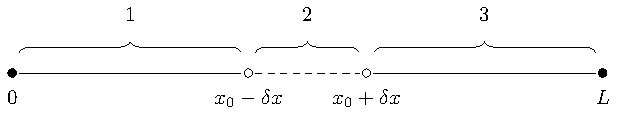
\includegraphics{figures/glitch-1d-example-diagram.pdf}
    \caption[A diagram showing a one-dimensional medium with a small structural perturbation.]{A diagram showing a one-dimensional medium split into three regions. 1: Fixed at \(x=0\) with a constant speed of sound \(c\); 2: A small structural perturbation centred at \(x=x_0\) with width \(2\delta x\) and constant speed of sound \(c + \delta c\); 3: Fixed at \(x=L\) with a constant speed of sound \(c\).}
    \label{fig:1d-diagram}
\end{figure}

Now, let us suppose there is a small structural perturbation (or glitch) in the medium at position \(x_0\) with half-width \(\delta x\). Figure \ref{fig:1d-diagram} shows this system divided into 3 regions, with region 2 containing the glitch. In region 2, the speed of sound is \(c + \delta c\) and the corresponding wave number is \(k + \delta k\). We want to find the frequencies which correspond to standing waves in this system and compare them to that of the homogeneous medium above. We will show that the resulting perturbation to the eigenfrequencies (\(\delta\omega\)) is periodic, with an amplitude and period that relates to the properties of the glitch.

Firstly, we propose solutions to the wave for each region by considering reflection and transmission at each boundary. Initially ignoring the wave superposed by a reflection at \(x=L\),
%
\begin{align}
    \xi_1(x, t) &= \ee^{i(\omega t - k x)} + A \ee^{i(\omega t + k x)}, \label{eq:xi1-r} \\
    \xi_2(x, t) &= B\ee^{i(\omega t - (k + \delta k) x)} + C \ee^{i(\omega t + (k + \delta k) x)}, \label{eq:xi2-r} \\
    \xi_3(x, t) &= D \ee^{i(\omega t - k x)}, \label{eq:xi3-r}
\end{align}
%
where complex coefficients \(A\) and \(C\) represent reflections, and \(B\) and \(D\) represent transmissions, at \(x_0 \pm \delta x\) respectively. Later, we will substitute the left-travelling wave (\(- \xi\{-k, -\delta k\}\)) after determining the values of the coefficients.

The internal boundary conditions for this system are found by enforcing spacial continuity at \(x - \delta x\) and \(x + \delta x\),
%
\begin{align*}
    \xi_1(x_0 - \delta x, t) &= \xi_2(x_0 - \delta x, t), \\
    \xi_2(x_0 + \delta x, t) &= \xi_3(x_0 + \delta x, t), \\
    \frac{\partial \xi_1}{\partial x}(x_0 - \delta x, t) &= \frac{\partial \xi_2}{\partial x}(x_0 - \delta x, t), \\
    \frac{\partial \xi_2}{\partial x}(x_0 + \delta x, t) &= \frac{\partial \xi_3}{\partial x}(x_0 + \delta x, t).
\end{align*}
%
Solving these simultaneously with the Python package \textsc{sympy} gives the following equations for the complex coefficients\footnote{The code for these derivations are available at \url{\gitremote/tree/\gitbranch/notebooks}},
%
\begin{align}
    A &= \delta k (2k + \delta k) (1 - \ee^{4i \delta x (k + \delta k)}) \ee^{- 2i k (x_0 - \delta x)} \alpha^{-1}, \\
    B &= 2 k (2k + \delta k) \ee^{4i \delta x (k + \delta k)} \ee^{i \delta k (x_0 - \delta x)} \alpha^{-1}, \\
    C &= 2 k \delta k \ee^{- i (x_0 - \delta x) (2k + \delta k)} \alpha^{-1}, \\
    D &= 4 k (k + \delta k) \ee^{2 i \delta x (2k + \delta k)} \alpha^{-1},
\end{align}
%
where,
\begin{equation}
    \alpha = (2k + \delta k)^2 \ee^{4 i \delta x (k + \delta k)} - \delta k^2.
\end{equation}
%

Now we have solutions for the coefficients, we can superpose the right-travelling wave, \(\xi\{k, \delta k\} \rightarrow - \xi\{-k, -\delta k\}\) to get the full solution for the wave function. Substituting \(k \rightarrow -k\) and \(\delta k \rightarrow -\delta k\) into the coefficients yields their complex conjugates, \((\overline{A},\overline{B},\overline{C},\overline{D})\). This allows us to rewrite the wave functions into a more flexible form. For example, substituting Euler's formula, \(A = (r_A/2) \ee^{i\phi_A}\) and \(\overline{A} = (r_A/2) \ee^{-i\phi_A}\), Equation \ref{eq:xi1-r} now becomes,
%
\begin{equation}
    \xi_1(x, t) = \ee^{i \omega t} \left[ \frac{r_A}{2} \left( \ee^{i(kx + \phi_A)} - \ee^{-i(kx + \phi_A)} \right) - \left( \ee^{ikx} - \ee^{-ikx} \right) \right] \label{eq:xi1}
\end{equation}
%
where its real component is,
\begin{equation}
    \real\left[\xi_1(x, t)\right] = \sin \omega t \left[2 \sin kx - r_A \sin(kx + \phi_A)\right].
\end{equation}
%
However, this does not satisfy the outer boundary condition that the displacement is always zero at \(x=0\); in other words, \(\xi_1(0, t) = - r_A \sin \omega t \sin(\phi_A) \neq 0\) everywhere. To fix this, we introduce a small displacement phase \(\epsilon\) caused by the glitch, and let \(x \rightarrow x + \epsilon\). We will determine \(\epsilon\) shortly. In the meantime, superposing the right-travelling wave and substituting Euler's formula into Equations \ref{eq:xi2-r} and \ref{eq:xi3-r}, we can write the real components of the wave functions,
%
\begin{align}
    \real[\xi_1(x, t)] &= \sin \omega t \left\{2 \sin[k (x + \epsilon)] - r_A \sin[k(x + \epsilon) - \phi_A]\right\} \label{eq:xi1-real} \\
    \real[\xi_2(x, t)] &= \sin \omega t \left\{ r_B \sin[(k + \delta k)(x + \epsilon) - \phi_B] - r_C \sin[(k + \delta k)(x + \epsilon) - \phi_C]\right\} \\
    \real[\xi_3(x, t)] &= \sin \omega t \left\{r_D \sin[k(x + \epsilon) - \phi_D]\right\} \label{eq:xi3-real}
\end{align}
%
Imposing the boundary condition \(\xi_1(0, t) = 0\), we solve Equation \ref{eq:xi1-real} for \(\epsilon\) at \(x=0\),
%
\begin{align}
    \epsilon &= \frac{1}{k} \tan^{-1}\left( \frac{(r_A / 2) \sin(\phi_A)}{1 - (r_A/2) \cos(\phi_A)} \right), \notag\\
    &= \frac{1}{k} \tan^{-1}\left( \frac{\imag[A]}{1 - \real[A]} \right). \label{eq:1d-phase}
\end{align}
%

Finally, we can impose the boundary condition \(\xi_3(L, t) = 0\) to solve for \(\omega\). Setting Equation \ref{eq:xi3-real} to zero, we can rewrite it in terms of the real and imaginary components of \(D\),
%
\begin{align}
    \sin \omega t \left\{r_D \sin[k(L + \epsilon) - \phi_D]\right\} &= 0, \quad (\div \sin \omega t) \notag \\
    r_D \cos \phi_D \sin[k(L + \epsilon)] - r_D \sin \phi_D \cos[k(L + \epsilon)] &= 0, \notag \\
    \real[D] \sin[k(L + \epsilon)] - \imag[D] \cos[k(L + \epsilon)] &=0. \label{eq:1d-glitch-sol}
\end{align}
%
The glitch affects the amplitude and phase of the wave. If we set \(\epsilon = 0\) and \(D = 1\) we recover the homogeneous frequency solutions (Equation \ref{eq:omega-n}). Unfortunately, solving Equation \ref{eq:1d-glitch-sol} for \(\omega\) is not possible analytically. However, we can find individual roots (or modes, \(\omega_n\)) numerically.

\begin{figure}[!tbp]
    \centering
    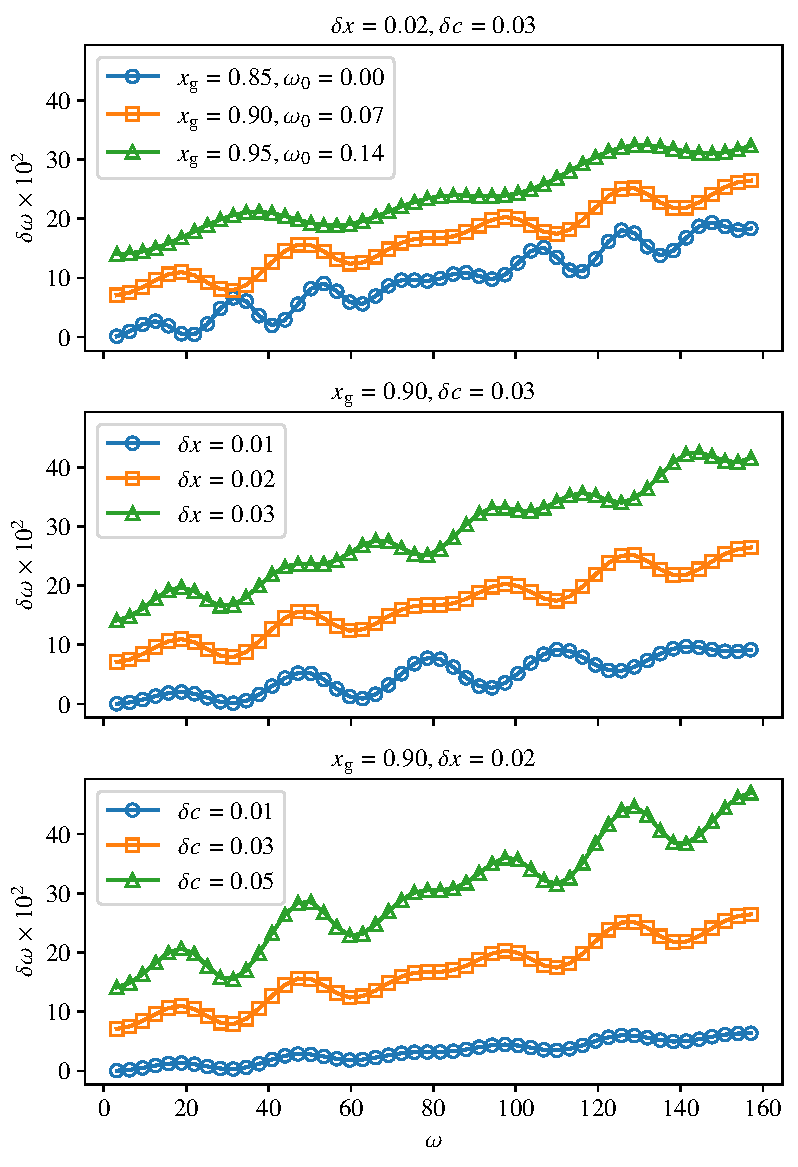
\includegraphics{figures/glitch-1d-example-results.pdf}
    \caption{The change in mode frequency induced by a change in sound speed of \(\delta c\) from \(x_0 - \delta x\) to \(x_0 + \delta x\) in a one-dimensional medium, bound such that \(x \in [0, 1]\) (see Figure \ref{fig:1d-diagram}). Outside of the perturbation the speed of sound, \(c=1\).
    The frequencies in the top panel are offset by \(\omega_0\).
    Points are joined by straight lines to guide the eye.
    }
    \label{fig:1d-results}
\end{figure}

We find \(\omega_n\) by solving Equation \ref{eq:1d-glitch-sol} using Newton's method for \(n = 1,\dots,50\). Using dimensionless units of length and time, we set \(c=1\), \(L=1\), and test several values of \(x_0\), \(\delta x\), and \(\delta c\). Initial guesses are obtained from the homogeneous medium solutions (\(\omega_n^0\)) in Equation \ref{eq:omega-n}. The difference between the solutions for \(\omega_n\) and those from the homogeneous medium, \(\delta \omega_n = \omega_n - \omega_n^0\), are shown in Figure \ref{fig:1d-results}. We can see an periodic component of \(\delta\omega\) induced by the glitch. Physically, this arises from the change in phase required to satisfy the boundary conditions of the glitch region. As the wave nodes pass in and out of the region with changing \(n\), the sensitivity of the wave to the glitch oscillates. The overall sensitivity to the glitch depends on how much the wave changes inside the glitch, hence why low \(n\) modes have smaller \(\delta\omega\).

The functional form of \(\delta\omega\) appears to have a linear component and a short period oscillation modulated by a longer period. As the location of the glitch (\(x_0\)) gets smaller, the short period of \(\delta\omega\) decreases. If we imagine the spacial distribution of nodes in the system as a function of \(n\), the density of nodes is larger towards the centre of the system. The periodicity arises from the nodes passing in and out of the glitch region with changing \(n\). Therefore, where the density of wave nodes is higher, we expect the short period of \(\delta\omega\) to decrease. Similarly, as the the half-width of the glitch (\(\delta x\)) increases, the longer period increases. 

Furthermore, an increasing change in sound speed (\(\delta c\)) increases the amplitude of \(\delta\omega\). This result is intuitive, as we expect a perturbation in \(c\) to be proportional to a perturbation in \(\omega\). Finally, increasing both \(\delta x\) and \(\delta c\) increases the slope of \(\delta\omega\). The sensitivity of a mode to the glitch increases with \(n\) and depends on how much the wave changes in the glitch region. A larger glitch allows modes of smaller \(n\) to `see' the glitch region, thus increasing the linear slope of \(\delta\omega\).

%This may be interpreted as the nodes of each standing wave passing in and out of region 2 with increasing \(n\). Where there is a node, the wave is least sensitive to a change in structure, and 

\begin{figure}[!tbp]
    \centering
    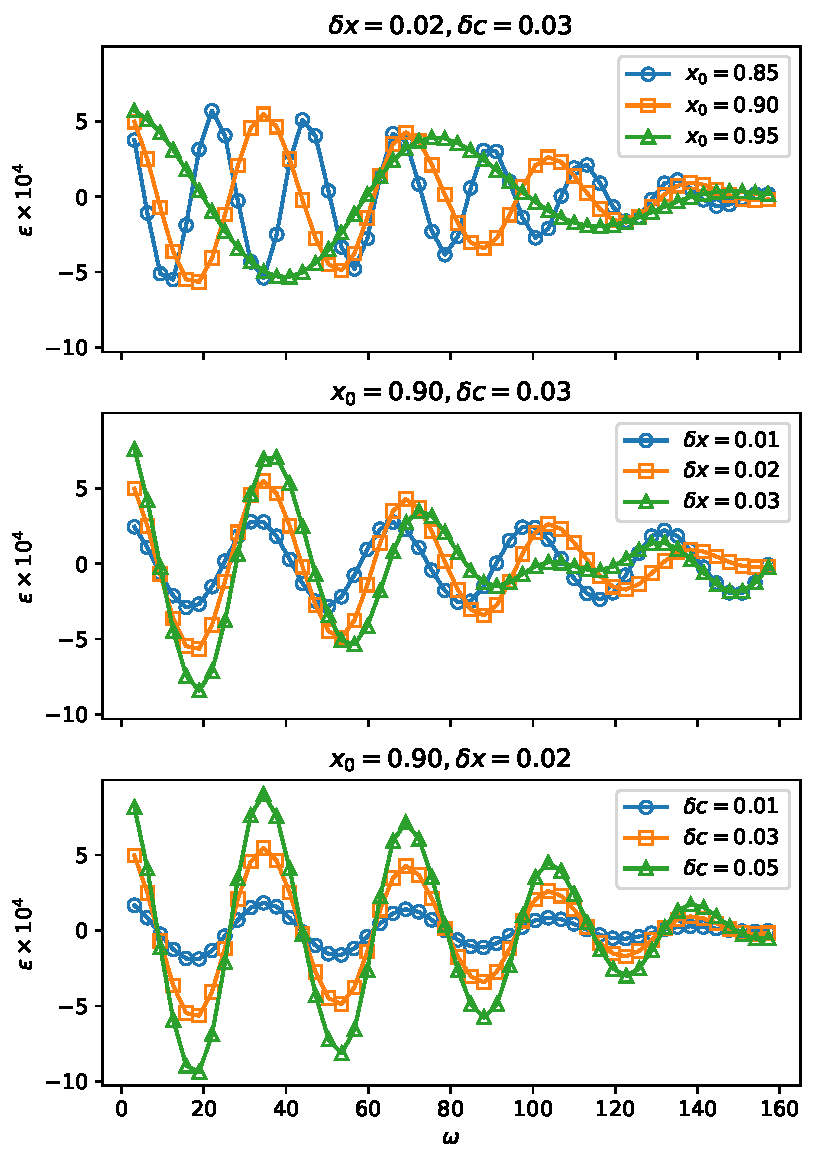
\includegraphics{figures/glitch-1d-example-phase.pdf}
    \caption{The same as Figure \ref{fig:1d-results} but showing the phase offset \(\epsilon\) required to satisfy the boundary conditions.}
    \label{fig:1d-phase}
\end{figure}

The small phase offset \(\epsilon\) in Equation \ref{eq:1d-phase} is required for the wave function to satisfy the boundary conditions at \(x = 0\). However, adding \(\epsilon\) shifts the effective location of \(x_0\) --- it changes the scale of the \(x\)-axis by a factor of \((1 + \epsilon)\). We plot \(\epsilon\) against \(\omega\) in Figure \ref{fig:1d-phase} and show that its magnitude is \(\sim 10^{-4}\), much smaller than the location and size of region 2. The periodicity caused by the glitch also shows up in Figure \ref{fig:1d-phase}, with its properties affected in a similar way to Figure \ref{fig:1d-results}.

Finding an approximate solution for \(\delta\omega\) is beyond the scope of this example. However, we can show that by modelling \(\delta\omega\), we can recover information about the structural glitch. Let us build a model \(\delta\omega = f(\omega)\). Looking at Figure \ref{fig:1d-results}, we propose a form for \(f\),
%
\begin{equation}
    f(\omega) = a_1 \omega - a_2 \sin (\tau_1 \omega) \cos (\tau_2 \omega), \label{eq:1d-domega-func}
\end{equation}
%
where \(a_1\) and \(a_2\) are coefficients which are both functions of \(\delta x\) and \(\delta c\). Parameters \(\tau_1\) and \(\tau_2\) are the `frequencies' (with dimensionless units of time\footnote{An angular frequency in \(\omega\)-space has units of time.}) of the periodic component to \(\delta\omega\), which are functions of \(\delta x\) and \(x_0\) respectively.

\begin{figure}[!tb]
    \centering
    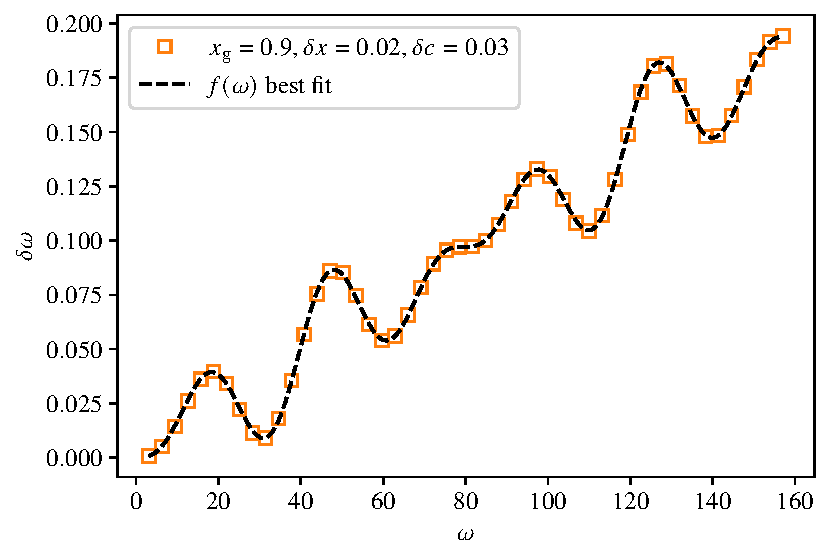
\includegraphics{figures/glitch-1d-fit.pdf}
    \caption{Best fit of Equation \ref{eq:1d-domega-func} to \(\delta\omega_n\) for \(n=1,\dots,50\), \(L=1\), and \(c=1\).}
    \label{fig:1d-fit}
\end{figure}

We fit Equation \ref{eq:1d-domega-func} to \(\delta\omega_n\) obtained from a glitch located at \(x_0 = 0.9\), with half-width \(\delta x = 0.02\), and change in sound speed \(\delta c = 0.03\). The best fitting line is shown in Figure \ref{fig:1d-fit}. We found \(\tau_1 \approx \num{0.0389}\) and \(\tau_2 \approx \num{0.199}\). This corresponded to \(\tau_1 \simeq 2\delta\tau\), where \(\delta\tau\) is half the acoustic width of the glitch --- the time at which sound takes to transverse the region. Since the speed of sound \(c \approx \num{1}\) throughout the medium, the true value of \(\delta\tau = 0.02\). We also found the second `frequency' \(\tau_2 \simeq 2\tau_0\), where \(\tau_0\) is the sound travel time from the nearest edge to the centre of the glitch (in this case \num{0.1}).

\todo{Repeating this for different glitch parameters,  how the `frequencies' \(\tau_1\) and \(\tau_2\) relate to the half-width and location of the glitch respectively.}

% NOTE: Could take this further to show a1 = 2 dc dtau / L and a2 = dc / L

It would not be hard to believe that a similar periodicity could be found in the mode frequencies of a star, although its structure is more complicated. We showed that fitting to \(\delta\omega\) we may can recover properties of a glitch. In the next section, we will build upon this analogy and explore acoustic glitches in stars.

% NOTES: Go slowly through this. The next step is to fit a simple mode to theses oscillations and show that we can find x0 and dx. And show how the amplitude scales with dc.

% NOTES: When it comes to fitting the helium glitch, consider first fitting a GP to the modes with a free noise term. Fix the kernel scale to a series of values and show that we can see the glitch in the residuals. Of course, this leaves the question of what kernel scale to use. Well, we could just model everything at once!

\section[Glitches in Stars]{Acoustic Glitches in Solar-Like Oscillators}\label{sec:glitch-star}

In the previous section, we considered a glitch in a homogeneous medium, where the speed of sound is constant everywhere else. In a star, the adiabatic sound speed is not constant. It depends on the density (\(\rho\)) and pressure (\(P\)),
%
\begin{equation}
    c^2 = \gamma \frac{P}{\rho},
\end{equation}
%
where \(\gamma \equiv \Gamma_1\) is the first adiabatic exponent,
%
\begin{equation}
    \gamma = \left( \frac{\partial \ln P}{\partial \ln \rho} \right)_S,
\end{equation}
%
at constant entropy, \(S\). \citet{Chandrasekhar1939} introduced three adiabatic exponents (\(\Gamma_1,\Gamma_2,\Gamma_3\)) to describe the non-ideal gas inside a star. However, in this chapter we do not use the other two and hence refer the first as \(\gamma\).

For the most part, \(\gamma\), \(P\), and \(\rho\) change smoothly with radius inside a star. However, a small structural glitch in these quantities would lead to a sudden change in sound speed. In the previous section, we showed how such a perturbation can lead to an periodic perturbation in the eigenfrequencies of pressure waves in a homogeneous medium. Characterising this signal allowed us to measure the properties of the glitch. If similar glitches were present in a star, then we might be able to do the same. In this section, we explore the origins of glitches inside a solar-like star. Then, we see what effect these have on the eigenfrequencies, a quantity we can measure through asteroseismology.

Firstly, let us consider the sound speed profile of a Sun-like star. Particularly, we want to see how the sound speed changes on the timescale of a pressure wave moving through the star. As discovered in Section \ref{sec:1d-glitch}, a convenient timescale to work with is the acoustic depth, \(\tau\). This is not to be confused with the symbol for the age of the star in Chapter \ref{chap:hmd}. Here, we define \(\tau\) as the time taken for a pressure wave to travel from its surface (\(R\)) to some radius \(r\) under the assumption of spherical symmetry,
%
\begin{equation}
    \tau(r) = \tau_0 - \int_0^{r} \frac{\dd r'}{c(r')},\label{eq:tau}
\end{equation}
%
where \(\tau_0\) is the acoustic radius of the star\footnote{Not to be confused with the glitch location in Section \ref{sec:1d-glitch}.}. We recall from Section \ref{sec:seismo} that \(\nu_0 \equiv (2\tau_0)^{-1}\) may be approximated by the large frequency separation (\(\Delta\nu_{nl}\)) in the asymptotic limit that \(l/n \rightarrow 0\).

\begin{figure}[!tb]
    \centering
    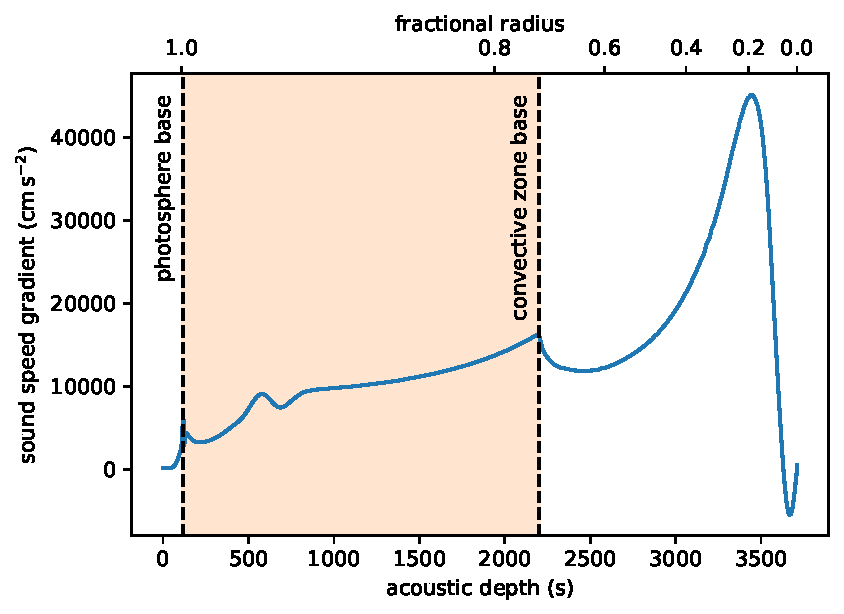
\includegraphics{figures/sound-speed-gradient.pdf}
    \caption{The sound speed gradient (\(\dd c/\dd \tau\)) of model S plot against the acoustic depth (\(\tau\)). The fractional radius to the photosphere base is given on the top axis. The convective envelope is shaded and the bases of the photosphere and convective zone are marked with dashed lines.}
    \label{fig:sound-speed-gradient}
\end{figure}

In Figure \ref{fig:sound-speed-gradient}, we show the sound speed gradient with respect to \(\tau\) for a Sun-like stellar model (model S; see Section \ref{sec:model-s}). We see how the speed of sound changes smoothly throughout the star. In the convective envelope, where p-modes propagate, there is a noticeable wiggle around \SI{700}{\second} and a sharp change in direction at its base. The first is caused by the ionisation of helium, which affects \(\gamma\) by increasing the number of free electrons and thus modifying the free energy of the gas. We explore this further in Section \ref{sec:helium-glitch}. The second is due to a discontinuity in the second temperature gradient as the structure moves from convectively unstable to radiative, which will be discussed in Section \ref{sec:bcz-glitch} \todo{Put a few references here of work which has studied these before}.

\subsection{Sun-Like Model Star}\label{sec:model-s}

We computed a representative Sun-like model star (hereafter model S) using MESA \citep[version 12115;][]{Paxton.Bildsten.ea2011,Paxton.Cantiello.ea2013,Paxton.Marchant.ea2015,Paxton.Schwab.ea2018,Paxton.Smolec.ea2019,Jermyn.Bauer.ea2023}. \todo{Insert details about physics used}. We output pulsation profile data in FGONG format to later use when computing oscillation modes in Section \ref{sec:glitch-model}.

\subsection{Helium Ionisation Glitch}\label{sec:helium-glitch}

In this section, we will first show how the sound speed inside a solar-like star is affected by the ionisation of hydrogen and helium. Then, we will see that an increase in helium abundance increases the effect of helium ionisation on the speed of sound. Starting with the variational principle, we derive a commonly used form of the glitch signature found in the mode frequencies. In the process, we show that the p modes are sensitive to changes in sound speed near the surface.

\begin{figure}[!tb]
    \centering
    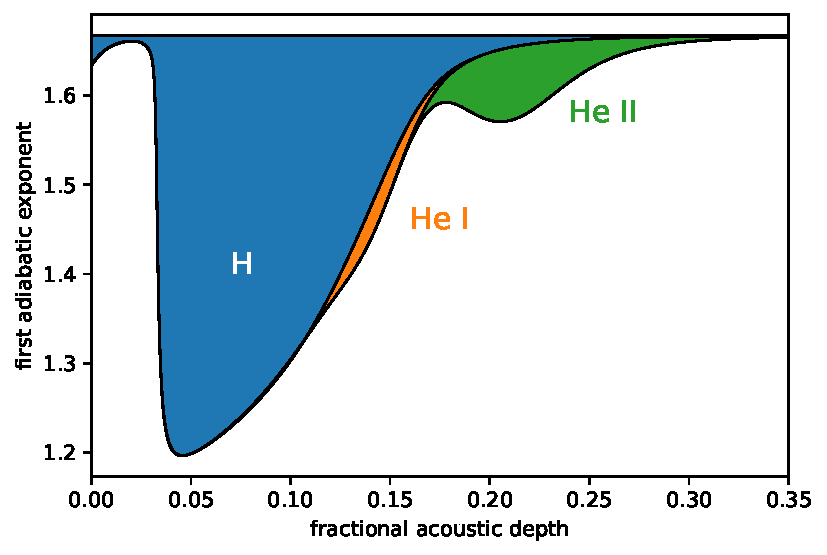
\includegraphics{figures/adiabatic-ionisation-regions.pdf}
    \caption[The depressions in the first adiabatic exponent caused by the ionisation of hydrogen and helium]{The depressions in the first adiabatic exponent (\(\gamma\)) caused by the ionisation of hydrogen (H), and the first and second ionisations of helium (He\,\textsc{i} and He\,\textsc{ii}). The horizonal axis is the fractional acoustic depth from the surface of the star, \(\tau/\tau_0\).}
    \label{fig:gamma-zones}
\end{figure}

The speed of sound in the star is proportional to \(\gamma\). As a chemical species in the star ionises, the number of particles and thus chemical potential of the species changes. This induces a gradient in the thermal free energy of the gas which relates to the pressure and entropy of the gas. Therefore, we expect ionisation to cause a change in the pressure-density gradient at constant entropy, \(\gamma\). Using an approximate form for the first adiabatic exponent, we show how \(\gamma\) is affected by the ionisation of helium and hydrogen in Figure \ref{fig:gamma-zones}. We see that hydrogen ionisation has the largest effect on \(\gamma\) close to the surface of the star. The first and second ionisations of helium occur deeper in the star, at higher temperatures. We can see that the second ionisation of helium has a greater affect on \(\gamma\) than the first. This is because the ionisation energy of He\,\textsc{ii} is higher than He\,\textsc{i} and the ground state degeneracy of He\,\textsc{ii} is less than He\,\textsc{i}.

\subsubsection{The Effect of Ionisation on \(\gamma\)}

The exact effect of ionisation on \(\gamma\) is not known analytically. However, \citet{Houdayer.Reese.ea2021} recently approximated \(\gamma\) for the convective zone of a Sun-like star in their study of the helium ionisation glitch. In this subsection, we combine the equations derived in their work to help us understand the relation between ionisation and \(\gamma\). Let us consider an \(M\) mass star with fractional hydrogen and helium abundances of \(X\) and \(Y\) respectively. From \citet{Houdayer.Reese.ea2021}, we approximate the first adiabatic exponent as,
%
\begin{equation}
    \gamma \simeq \frac{5}{3} - \frac{2}{3} \, \eta(T, \rho), \label{eq:gamma1}
\end{equation}
%
where \(\eta\) represents the depression in \(\gamma\). Considering a hydrogen-helium mixture where \(X + Y \approx 1\), \(\eta\) is,
%
\begin{equation}
    \begin{split}
        \eta(T, \rho) &= \frac{1}{\partial_{TT}^2 f} \left[n_\hydrogen y_\hydrogen \, (1 - y_\hydrogen) \, \frac{(\chi_\hydrogen / k_B T)^2}{2 - y_\hydrogen}
        % \right. \\ &\left. 
        + n_\helium y_\helium^{(1)} \left(1 - y_\helium^{(1)}\right) \left(\frac{\chi_\helium^{(1)}}{k_B T}\right)^2 
        \right. \\ &\left.
        + \, n_\helium y_\helium^{(2)} \left(1 - y_\helium^{(2)}\right) \left(\frac{\chi_\helium^{(2)}}{k_B T}\right)^2\right],
    \end{split}
\end{equation}
%
where \(k_B\) is the Boltzmann constant. The parameter \(\partial_{TT}^2\) is the second partial derivative of the free energy density with respect to temperature (\(T\)),
%
\begin{equation}
    \begin{split}
        \partial_{TT}^2 f &\simeq \frac{3}{2} + n_\hydrogen y_\hydrogen \left[ \frac{3}{2} + \frac{(1 - y_\hydrogen)}{2 - y_\hydrogen} \left(\frac{3}{2} + \frac{\chi_\hydrogen}{k_B T}\right)^2 \right] %\\
        + n_\helium y_\helium^{(1)} \left[ \frac{3}{2} + \left(1 - y_\helium^{(1)}\right) \left(\frac{3}{2} + \frac{\chi_\helium^{(1)}}{k_B T}\right)^2 \right] \\
        &+ n_\helium y_\helium^{(2)} \left[ \frac{3}{2} + \left(1 - y_\helium^{(2)}\right) \left(\frac{3}{2} + \frac{\chi_\helium^{(2)}}{k_B T}\right)^2 \right],
    \end{split}
\end{equation}
%
where \(n_\mathbb{X} = N_\mathbb{X} / N\) is the number density and \(\chi_\mathbb{X}^{i}\) is the \(i\)-th ionisation energy of species \(\mathbb{X}\). Parameter \(y_\mathbb{X}^i\) is related to a reduced form of Saha's equation \needcite,
%
\begin{equation}
    \frac{(y_\mathbb{X}^i)^q}{1 - y_\mathbb{X}^i} = \frac{2 g_\mathbb{X}^i}{g_\mathbb{X}^{i-1}} \frac{\overline{m}}{\rho \lambda_\ee^3} \, \ee^{- \chi_\mathbb{X}^i / k_B T},
\end{equation}
%
where \(q = 2\) for hydrogen, \(q = 1\) for helium, \(\overline{m} = M/N\) is the mean mass, and \(g_\mathbb{X}^i\) is the ground-state degeneracy of ionisation state \(i\). We used these equations to produce Figures \ref{fig:gamma-zones} and \ref{fig:gamma-temp-density}.

\begin{figure}[tbp]
    \centering
    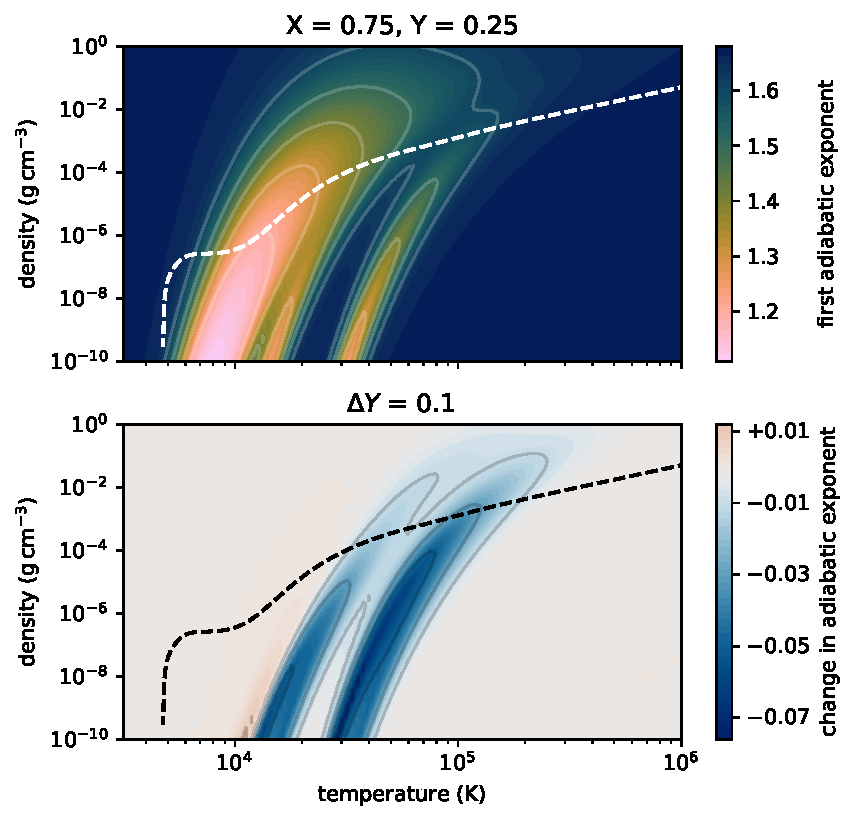
\includegraphics{figures/adiabatic-ionisation-temp.pdf}
    \caption{Temperature-density profile of a Sun-like star. \emph{Top:} The first adiabatic exponent \(\gamma\) as a function of temperature and density, calculated using Equation \ref{eq:gamma1} for a helium mass fraction, \(Y=0.25\). \emph{Bottom:} The change in \(\gamma\) induced by a change in helium abundance, \(\Delta Y = 0.1\). In both panels, the dashed line shows the temperature-density profile of model S.}
    \label{fig:gamma-temp-density}
\end{figure}

In Figure \ref{fig:gamma-temp-density} we plot \(\gamma\) as a function of pressure and temperature. The first panel illustrates the three ionisation regions of hydrogen and helium. The value of \(\gamma\) decreases when the ionisation reaction is occurring. The magnitude of the effect depends primarily on the temperature-density profile of the star. Additionally, in the second panel we see that an increase in helium abundance decreases \(\gamma\) in the helium ionisation regions. A temperature-density profile from model S is shown to see how the star probes the ionisation regions. We can imagine a hotter star shifting this line such that ionisation occurs closer to the surface. Similarly, the effect on \(\gamma\) would be smaller in denser star. Although helium abundance dominates the effect on \(\gamma\), there is still some dependence on other stellar quantities.

\subsubsection{The Effect of \(\gamma\) on p Mode Frequencies}

\begin{figure}[tbp]
    \centering
    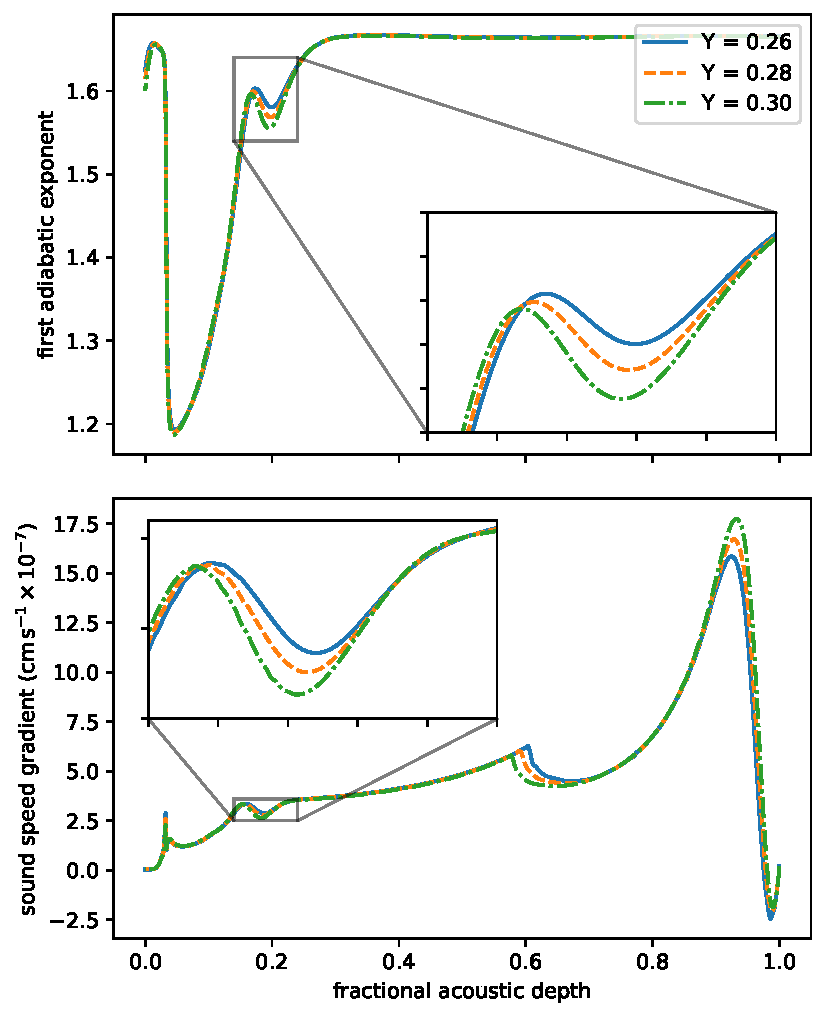
\includegraphics{figures/helium-ionisation-sound-speed.pdf}
    \caption{The effect on the sound speed profile for three solar-like stars with initial helium mass fractions of 0.26 (\emph{solid}), 0.28 (\emph{dashed}), and 0.3 (\emph{dot-dashed}). The models were each evolved to a central helium mass fraction of 0.6. \emph{Top:} The first adiabatic exponent \(gamma\). \emph{Bottom:} The sound speed gradient \(\dd c/\dd t\) where \(t = \tau/\tau_0\) is the fractional acoustic depth (plot on the x-axis).}
    \label{fig:gamma-sound-speed}
\end{figure}

To show the effect of small changes in \(\gamma\) on the sound speed, we plot the sound speed gradient in Figure \ref{fig:gamma-sound-speed}. The three models shown were evolved to the same central temperature with different initial helium abundances. The dominant effect of helium abundance appears as a Gaussian-like depression in \(\gamma\) around the second ionisation of helium. We see how larger helium abundance increases the width and depression in \(\gamma\), which is reflected in the sound speed gradient. A larger \(Y\) also leads to a relative reduction in hydrogen abundance. This slightly shrinks the width of the hydrogen ionisation region.

To see how a change in \(\gamma\) affects the mode frequencies, we will consider the sensitivity of a given mode to structural changes in the star. We can get there by starting with the variational principle \citep{Chandrasekhar1964},
%
\begin{equation}
    \omega^2 = \frac{\mathcal{E}}{\mathcal{I}}\label{eq:var-prin}
\end{equation}
%
which approximates the characteristic frequencies of a spherically symmetric, slowly rotating star as a function of the mode inertia,
%
\begin{equation}
    \mathcal{I} = \int_0^R \vect{\xi} \cdot \vect{\xi} \, \rho r^2 \, \dd r
\end{equation}
%
and \(\mathcal{E}\) which is proportional to the mode energy,
%
\begin{equation}
    \mathcal{E} = \int_0^R \left[\gamma P (\dive{\vect{\xi}})^2 + 2(\vect{\xi}\cdot \nabla P) \dive{\vect{\xi}} + (\vect{\xi}\cdot \nabla P) (\vect{\xi}\cdot\nabla\ln\rho)\right] r^2 \, \dd r.
\end{equation}
%
These equations depend on \(\vect{\xi}\), the Lagrangian perturbation vector of the pulsation mode (the amplitude and direction of the wave). \todo{Explain the meaning of each term}. A structural glitch in the star would cause a small change in frequency (\(\delta\omega\)). Differentiating both sides of Equation \ref{eq:var-prin} with respect to \(\omega\), we get,
%
\begin{align}
    2\omega &= \frac{1}{\mathcal{I}} \left( \frac{\delta\mathcal{E}}{\delta\omega} - \omega^2 \frac{\delta\mathcal{I}}{\delta\omega}\right), \qquad \left[\times \frac{\delta\omega}{2\omega^2}\right] \notag \\
    \frac{\delta\omega}{\omega} &= \frac{1}{2\,\mathcal{I}} \left(\frac{\delta\mathcal{E}}{\omega^2} - \delta\mathcal{I}\right).
\end{align}
%
The perturbations \(\delta\mathcal{E}\) and \(\delta\mathcal{I}\) depend on changes in the state variables. To see the effect of a change in structure on the modes, it is possible to rewrite this as a function of the so-called structural kernels \(\mathcal{K}_{a,b}\), for example,
%
\begin{equation}
    \frac{\delta\omega}{\omega} = \int_0^R \left(\mathcal{K}_{c^2,\rho} \frac{\delta c^2}{c^2} + \mathcal{K}_{\rho,c^2} \frac{\delta \rho}{\rho} \right) \dd r.\label{eq:kernels}
\end{equation}
%
where \(\mathcal{K}_{a, b}\) gives the relative effect on \(\omega\) due to a perturbation in a state variable \(a\) at fixed \(b\), at a given \(r\). These kernels are defined fully in \citet{Gough.Thompson1991}.

\begin{figure}[!tbp]
    \centering
    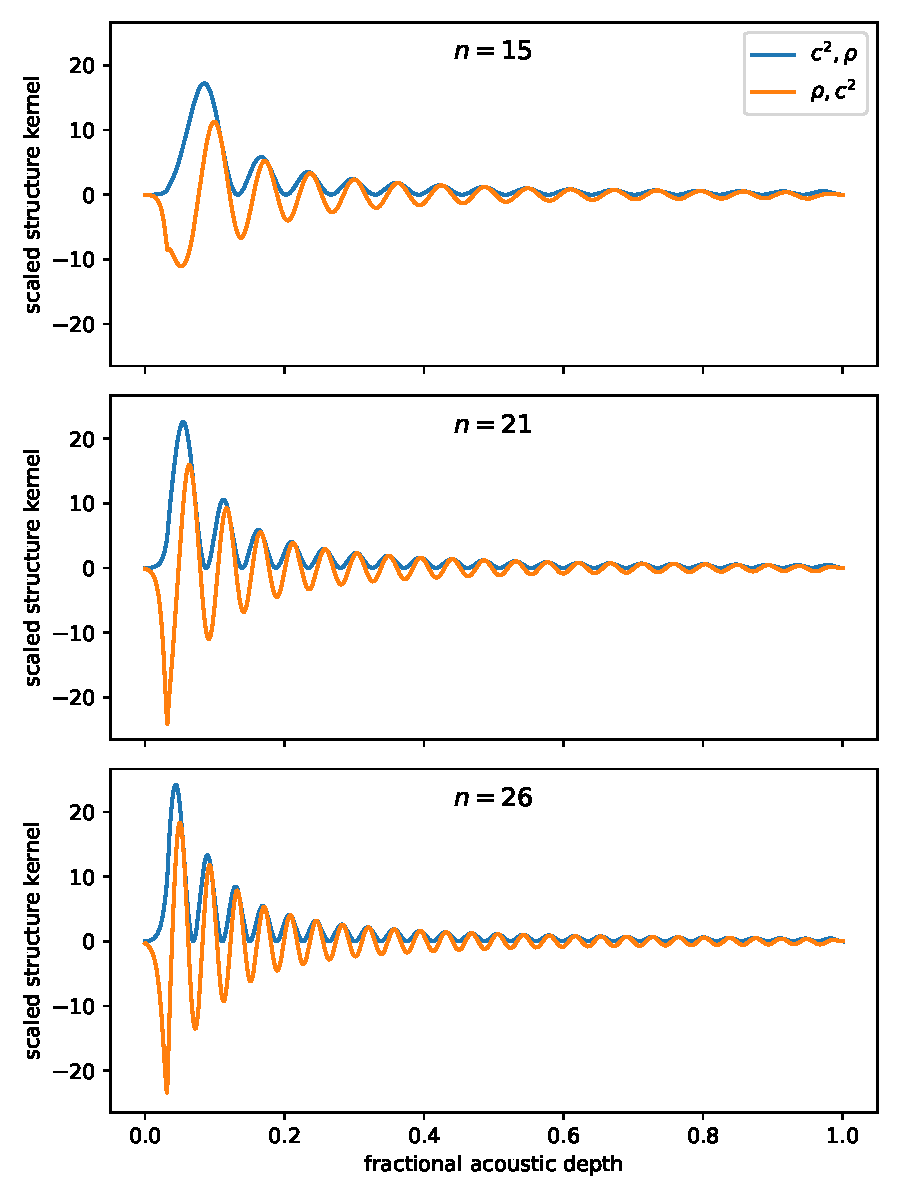
\includegraphics{figures/kernels.pdf}
    \caption{Structure kernels (\(\mathcal{K}_{c^2,\rho}, \mathcal{K}_{\rho,c^2}\)) scaled by the stellar radius as a function of fractional acoustic depth. The kernels were computed for three radial oscillation modes (\(n=15,21,26\)) using oscillation calculations for stellar model S.}
    \label{fig:kernels}
\end{figure}

We plot examples of these kernels in Figure \ref{fig:kernels} for a few radial oscillation modes. Both decay through the star, meaning that the modes are less sensitive to structural changes deeper in the star. The second term of Equation \ref{eq:kernels} is approximately zero, unless there is a sharp change in \(\delta\rho/\rho\) (such as at the base of the convective zone). Also, the first kernel \(\mathcal{K}_{\gamma,\rho} \equiv \mathcal{K}_{c^2,\rho}\) because \(c^2 \propto \rho\). Therefore, we may rewrite Equation \ref{eq:kernels} as
%
\begin{equation}
    \frac{\delta\omega}{\omega} \simeq \int_0^R \mathcal{K}_{\gamma,\rho} \frac{\delta\gamma}{\gamma} \dd r,\label{eq:delta-omega}
\end{equation}
%
where \(\mathcal{K}_{\gamma,\rho}\) is shown in \citet{Gough1993} to satisfy,
%
\begin{equation}
    \omega^2 \mathcal{I}\mathcal{K}_{\gamma,\rho} = \frac12 \gamma P (\dive{\vect{\xi}})^2 r^2.\label{eq:gamma-kernel}
\end{equation}
%
\todo{} show how this gets to, using equations for \(\xi_r\) and pressure perturbation \(P'\) from eq. 24-25 of e.g. \citet{Shibahashi1979}, \(\vect{\xi} = \xi_r \hat{r} + \vect{\xi}_h\) for high-order acoustic modes (where we can ignore the horizontal component of \(\vect{\xi}\)).
%
\begin{equation}
    \xi_r \simeq \frac{\psi_0}{r}\sqrt{\frac{K}{\rho}} \cos\psi,\qquad
    (\dive{\vect{\xi}})^2 \simeq \frac{\psi_0^2 \omega^3}{\gamma P c r^2} \sin^2\psi, \label{eq:xi-approx}
\end{equation}
%
where \(\psi_0\) is a proportionality constant and the radial wave number \(K \simeq \omega / c\) for high-order acoustic modes. The phase term \(\psi \simeq \omega \tau + \epsilon\) when \(\tau\) is not close to the upper turning point (where the wave is reflected near the stellar surface), and the small offset \(\epsilon\) is a slowly varying function of \(\tau\).

\begin{align}
    \mathcal{I} &\simeq \int_0^R \xi_r^2 \rho r^2 \, \dd r \notag\\
    &\simeq \psi_0^2 \int_0^R K \cos^2\psi \, \dd r \notag \\
    &= \frac12 \omega \psi_0^2 \int_0^R (1 + \cos 2 \psi) \frac{\dd r}{c}
\end{align}
%
Changing to an integral over acoustic depth we can evaluate it for high-order modes where \(\omega_n \ll \tau_0^{\,-1}\),
%
\begin{align}
    \mathcal{I} &\simeq \frac12 \omega \psi_0^2 \int_0^{\tau_0} [1 + \cos 2 (\omega\tau + \epsilon)] \, \dd \tau \simeq \frac12 \omega \psi_0^2 \tau_0.
\end{align}
%
Finally, substituting Equations \ref{eq:gamma-kernel} and \ref{eq:xi-approx} into Equation \ref{eq:delta-omega}, we get,
%
\begin{align}
    \frac{\delta\omega}{\omega} &\simeq \frac{1}{2\omega^2\mathcal{I}} \int \delta\gamma P (\dive{\vect{\xi}})^2 r^2 \, \dd r, \notag \\
    &\simeq \frac{\omega \psi_0^2}{2 \mathcal{I}} \int \frac{\delta\gamma}{\gamma}\sin^2\psi\frac{\dd r}{c}, \notag \\
    &= \frac{\omega \psi_0^2}{4 \mathcal{I}} \int \frac{\delta\gamma}{\gamma}(1 - \cos 2\psi)\frac{\dd r}{c}.
\end{align}
%
where the integral need only be evaluated in the region where \(\delta\gamma / \gamma\) is non-zero. We can see that \(\delta\omega\) is split into a smooth and a periodic component. The smooth component may be treated later, but for now we focus on the oscillating part of \(\delta\omega\). Substituting for \(\mathcal{I}\) and \(\psi\), changing to an integral over acoustic depth we get,
%
\begin{equation}
    \left.\frac{\delta\omega}{\omega}\right|_\mathrm{osc} \simeq - \frac{1}{2\tau_0} \int \frac{\delta\gamma}{\gamma} \cos 2 (\omega\tau + \epsilon) \, \dd \tau,
\end{equation}
%

\subsubsection{A Functional Form of the Helium Glitch Signature}

We have shown that a perturbation in \(\gamma\) can induce an periodicity in \(\omega\). The functional from of this periodicity depends on \(\delta\gamma/\gamma\). As shown in Figures \ref{fig:gamma-zones} and \ref{fig:gamma-temp-density}, the dominant perturbation due to a change in helium abundance is from the second ionisation of helium. There have been different attempts to approximate \(\delta\gamma/\gamma\,|_\heII\) in the literature, for example using a Dirac delta function or a triangular function \citep{Monteiro.Christensen-Dalsgaard.ea1994, Monteiro.Thompson2005}. In recent years, work modelling the glitch has used the formulation from \citet{Houdek.Gough2007} where the perturbation is modelled with a Gaussian shape,
%
\begin{equation}
    \left.\frac{\delta\gamma}{\gamma}\right|_\heII \simeq - \frac{\Gamma_\heII}{\Delta_\heII \sqrt{2\pi}} \, \ee^{- \frac12{(\tau - \tau_\heII)^2}/{\Delta_\heII^2} }, \label{eq:he-gamma}
\end{equation}
%
where \(\Gamma_\heII\) is the area, \(\Delta_\heII\) is the characteristic width, and \(\tau_\heII\) is the center of the ionisation region.

Combine the above two equations with a change of variables to \(x = (\tau - \tau_\heII)/\Delta_\heII\), we get,
%
\begin{equation}
    \left.\frac{\delta\omega}{\omega}\right|_{\heII, \mathrm{osc}} \simeq \frac{\Gamma_\heII}{2\sqrt{2\pi} \, \tau_0} \, \int_{-\infty}^\infty \ee^{- x^2/2} \cos 2 (\Delta_\heII \omega x + \widetilde{\epsilon_\heII}) \, \dd x
\end{equation}
%
where \(\widetilde{\epsilon_\heII} = \omega\tau_\heII + \epsilon_\heII\) and the phase \(\epsilon=\epsilon_\heII\) is assumed constant accross the glitch region. We can solve the above integral analytically using differentiation under the integral sign by introducing an arbitrary variable \(a\),
%
\begin{equation}
    I(a) = \int_{-\infty}^\infty \ee^{- x^2/2 } \cos 2 (\Delta_\heII \omega x a + \widetilde{\epsilon_\heII}) \, \dd x
\end{equation}
%
Differentiating this with respect to \(a\), and then integrating by parts gets,
%
\begin{align}
    I'(a) &= - 2 \Delta_\heII \omega \int_{-\infty}^\infty x \, \ee^{- x^2/2 } \sin 2 (\Delta_\heII \omega x a + \widetilde{\epsilon_\heII}) \, \dd x, \notag\\
    &= - 2 \Delta_\heII \omega \int_{-\infty}^\infty \sin 2 (\Delta_\heII \omega x a + \widetilde{\epsilon_\heII}) \, \dd \ee^{- x^2/2 }, \notag\\
    &= 2 \Delta_\heII \omega \left\{ \left[ \ee^{- x^2/2 } \sin 2 (\Delta_\heII \omega x a + \widetilde{\epsilon_\heII}) \right]_{-\infty}^\infty - 2 \Delta_\heII \omega a \int_{-\infty}^\infty \ee^{- x^2/2 } \cos 2 (\Delta_\heII \omega x a + \widetilde{\epsilon_\heII}) \, \dd x \right\}, \notag\\
    &= - 4 \Delta_\heII^2 \omega^2 a \, I(a),
\end{align}
%
which is a differential equation with the solution,
%
\begin{equation}
    \begin{split}
        I(a) = I(0) \ee^{- 2 \Delta_\heII^2 \omega^2 a^2}, \qquad I(0) &= \int_{-\infty}^\infty \ee^{- x^2/2 } \cos 2 \widetilde{\epsilon_\heII} \, \dd x, \\
        &= \sqrt{2\pi} \, \cos 2 \widetilde{\epsilon_\heII},
    \end{split}
\end{equation}
%
Therefore, if we set \(a = 1\) for the case of the integral in Equation \ref{} we get the following for the periodic glitch signature \citep[cf.][]{Houdek.Gough2007},
%
\begin{equation}
    \left.\frac{\delta\omega}{\omega}\right|_{\heII, \mathrm{osc}} \simeq \frac{\Gamma_\heII}{2 \tau_0} \ee^{- 2 \Delta_\heII^2 \omega^2} \cos 2 (\tau_\heII\omega + \epsilon_\heII),
\end{equation}
%
To get this in a more familiar form in terms of cyclic frequency \citep[e.g.][]{Verma.Faria.ea2014,Verma.Raodeo.ea2017}, we substitute \(\omega = 2\pi\nu\),
%
\begin{equation}
    \left.\frac{\delta\nu}{\nu}\right|_{\heII, \mathrm{osc}} \simeq \nu_0 \Gamma_\heII \, \ee^{- 8 \pi^2 \Delta_\heII^2 \nu^2} \, \sin ( 4 \pi \tau_\heII \nu + \phi_\heII), \label{eq:he-osc}
\end{equation}
%
where \(\phi_\heII = 2(\epsilon_\heII + \pi/4)\), and \(\nu_0 = (2 \tau_0)^{-1}\) is the inverse acoustic diameter of the star.

\subsection{Base of the Convective Zone Glitch}\label{sec:bcz-glitch}

The sensitivity of p-modes to glitches gets smaller further into the star. However, we should not neglect the effect of a discontinuity at the base of the convective zone. This arises 

\begin{figure}[!tb]
    \centering
    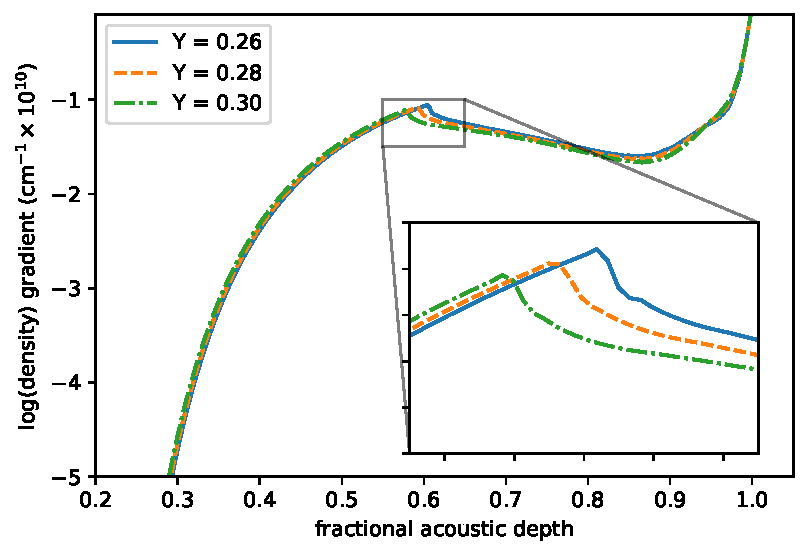
\includegraphics{figures/bcz-density-gradient.pdf}
    \caption{Discontinuity in the density gradient at the base of the convective zone for three solar-like stars with initial helium mass fractions of 0.26 (\emph{solid}), 0.28 (\emph{dashed}), and 0.3 (\emph{dot-dashed}).}
    \label{fig:bcz-density}
\end{figure}


We can take a similar approach to the previous section but now considering the second kernel \(\mathcal{K}_{\rho,c^2}\) in Equation \ref{eq:kernels}. However, \citet{Houdek.Gough2007} take another approach by considering the discontinuity as it appears in the acoustic cut-off frequency, \(\omega_{ac}\). The details of this derivation are beyond the scope of this work. We quote their result for the change in frequency induced by a density discontinuity at the base of the convective zone located at an acoustic depth of \(\tau_\bcz\),
%
\begin{equation}
    \left.\frac{\delta\omega}{\omega}\right|_{\bcz,\mathrm{osc}} \simeq \frac{c_\bcz^2\Delta_\bcz}{8\tau_0 \omega^3} \left(1 + {1}/{4\tau_0^2\omega^2}\right)^{-1/2} \cos\left[2(\tau_\bcz \omega + \epsilon_\bcz) + \tan^{-1}(2\tau_0\omega)\right]
\end{equation}
%
where \(\epsilon_\bcz\) is some phase which depends slowly on \(\omega\), \(c_\bcz\) is the speed of sound and,
%
\begin{equation}
    \Delta_\bcz = \left[\frac{\dd^2 \ln\rho}{\dd r^2}\right]_{-r_\bcz}^{+r_\bcz},
\end{equation}
%
is the change in second derivative of density at the base of the convective zone (\(r = r_\bcz\)).

For high-order modes, \(\tau_0 \omega \gg 1\) and thus \(\tan^{-1}(2\tau_0\omega) \simeq \pi/2\), and \((1 + {1}/{4\tau_0^2\omega^2})^{-1/2} \simeq 1\). Therefore, we can simplify this and write it in a more familiar form in terms of cyclic frequency,
%
\begin{equation}
    \left.\frac{\delta\nu}{\nu}\right|_{\bcz,\mathrm{osc}} \simeq \frac{c_\bcz^2\Delta_\bcz\nu_0}{32\pi^3 \nu^3} \sin(4\pi\tau_\bcz\nu + \phi_\bcz) \label{eq:bcz-osc}
\end{equation}
%
where \(\phi_\bcz\) is some approximately constant phase term.

\section[Modelling the Glitch]{Modelling Glitches in Stellar Oscillations}\label{sec:glitch-model}

Let us consider a non-rotating star which oscillates at frequencies \(\nu_{nl}\), where \(n\) and \(l\) are the radial order and angular degree of the modes. We may model the modes as the sum of a smoothly-varying component, \(\tilde{f}(n, l)\), and quickly-varying, small change in frequency, \(\delta\nu\), arising from glitches in the stellar structure,
%
\begin{equation}
    f(n, l) = \tilde{f}(n, l) + \delta\nu,\label{eq:general-glitch}
\end{equation}
%
where \(\delta\nu\) is some function of frequency which may, for example, be evaluated at \(\tilde{f}(n, l)\).

In principle, \(\delta\nu\) could arise from any glitches expected for a particular star. For this work, we consider glitches in main sequence solar-like oscillators. Previously, we derived approximations for \(\delta\nu\) arising from acoustic glitches caused by the second ionisation of helium and the BCZ. Here, we choose to ignore contributions to \(\delta\nu\) from the first ionisation of helium. As a result, we let \(\delta\nu = \delta\nu_\helium + \delta\nu_\bcz\) where each component depends on parameters relating to properties of the glitches (cf. Equations \ref{eq:he-osc} and \ref{eq:bcz-osc}),
%
\begin{align}
    \delta\nu_\helium &= \alpha_\helium \nu_0 \nu \, \ee^{-\beta_\helium \nu^2} \sin(4\pi\tau_\helium\nu + \phi_\helium), \label{eq:he-glitch}\\
    \delta\nu_\bcz &= \alpha_\bcz \nu_0 \nu^{-2} \, \sin(4\pi\tau_\bcz\nu + \phi_\bcz). \label{eq:bcz-glitch}
\end{align}
%
The parameters \(\alpha_\helium \cong \Gamma_\heII\) and \(\beta_\helium \propto \Delta_\heII^2\) relate to the area and variance of the Gaussian-like depression in \(\gamma\) caused by the second ionisation of helium. The amplitude parameter for the BCZ glitch, \(\alpha_\bcz \propto \Delta_{\bcz}\) is proportional to the difference in the second density derivative at the base of the convective zone and has units of frequency squared. The approximate acoustic depths of second helium ionisation and the BCZ are given by \(\tau_\helium\) and \(\tau_\bcz\) respectively, and \(\phi\) represents an arbitrary phase constant.

Providing \(\tilde{f}(n, l)\) is a good approximation of the mode frequencies, we can calculate \(\delta\nu\) at \(\nu = \tilde{f}(n, l)\) to predict \(f(n, l)\). For example, \(\tilde{f}(n,l)\) could be a \(K\)-th order polynomial in \(n\) with coefficients \(a_{lk}\) \citep[e.g.][]{Kjeldsen.Bedding.ea2005,Ulrich1986},
%
\begin{equation}
    \tilde{f}(n, l) = \nu_0 \sum_{k=0}^{K} a_{lk} n^k. \label{eq:poly}
\end{equation}
%
The linear component of this is equivalent to the asymptotic expression (cf. Equation \ref{}) and the remaining terms describe curvature in the mode frequencies \todo{refer to earlier echelle plot}. However, there are drawbacks to using a polynomial for \(\tilde{f}(n, l)\). Whilst a polynomial with \(K = \infty\) can represent any function, this is impractical here. If \(K\) is too low, then it will not be flexible enough, biasing \(\delta\nu_\helium\) and \(\delta\nu_\bcz\). Yet, if \(K\) is too high, then it will over-fit and the glitch component may be missed. Regularising the polynomial is one solution to over-fitting, but this adds extra parameters to tune. Additionally, a finite polynomial represents only a small fraction of function space, leading to our model to be systematically biased to a particular functional form of \(\tilde{f}\).

\defcitealias{Verma.Raodeo.ea2019}{V19}

Directly fitting the glitch the above way has been done before \citep[e.g.][]{Verma.Faria.ea2014,Verma.Raodeo.ea2017,Mazumdar.Monteiro.ea2014}. In this work, we will compare the most recent version of this method \citep[][hereafter V19]{Verma.Raodeo.ea2019} with a new method defined in this work. Our method will make use of a Gaussian Process to marginalise over our uncertainty in the functional form of \(f\). In the next section, we introduce the data used in comparing the two methods. Then, we define both modelling methods being compared in Section \ref{sec:glitch-methods}. Finally, we apply the methods to the data and present the results and discussion in Sections \ref{sec:glitch-results} and \ref{sec:glitch-disc}.

\subsection{Data}\label{sec:glitch-data}

In this section, we briefly outline the data used to compare our new method with the \citetalias{Verma.Raodeo.ea2019} method. For simplicity, we only use observations of radial mode frequencies in this work. However, both methods can be extended to use higher-order modes.

\begin{table}
    \centering
    \caption{Observations of radial mode frequency \(\nu_n\) at radial order \(n\) for model star S (\emph{left}) and 16 Cyg A (\emph{right}). \(N\) are the number of observed radial orders and the scale of the Gaussian noise added to each column is given by \(\sigma_\obs\) where appropriate. The values and their uncertainties for 16 Cyg A come from \citet{Lund.SilvaAguirre.ea2017}.}
    \label{tab:glitch-obs}
    \begin{tabular}{ccccc}
\toprule
Case & Worst & Better & Best & Truth \\
$N, \sigma_n$ & 6, 1.00 & 12, 0.10 & 18, 0.01 &  \\
$n$ &  &  &  &  \\
\midrule
12 & --- & --- & 1781.726 & 1781.729 \\
13 & --- & --- & 1914.348 & 1914.330 \\
14 & --- & --- & 2047.296 & 2047.314 \\
15 & --- & 2180.16 & 2180.107 & 2180.125 \\
16 & --- & 2312.00 & 2312.030 & 2312.029 \\
17 & --- & 2442.64 & 2442.807 & 2442.808 \\
18 & 2577.2 & 2574.32 & 2574.260 & 2574.263 \\
19 & 2706.4 & 2706.50 & 2706.612 & 2706.596 \\
20 & 2839.0 & 2839.46 & 2839.446 & 2839.476 \\
21 & 2971.5 & 2972.92 & 2972.718 & 2972.727 \\
22 & 3107.4 & 3105.77 & 3105.749 & 3105.759 \\
23 & 3240.0 & 3239.18 & 3239.177 & 3239.175 \\
24 & --- & 3372.94 & 3372.980 & 3372.990 \\
25 & --- & 3507.22 & 3507.115 & 3507.112 \\
26 & --- & 3641.56 & 3641.715 & 3641.702 \\
27 & --- & --- & 3776.339 & 3776.350 \\
28 & --- & --- & 3911.281 & 3911.279 \\
29 & --- & --- & 4046.319 & 4046.312 \\
\bottomrule
\end{tabular}

\end{table}

\begin{figure}[!tb]
    \centering
    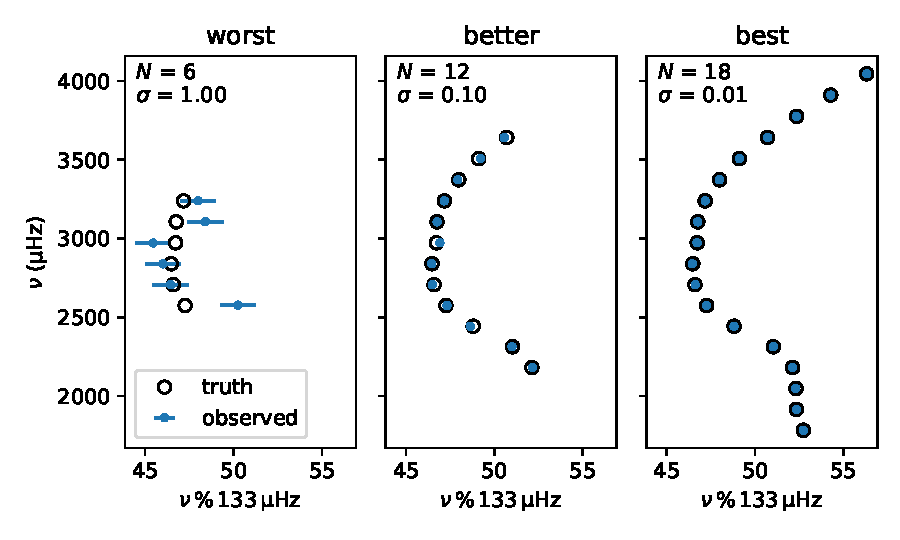
\includegraphics{figures/glitch-test-obs.pdf}
    \caption{Echelle plot of simulated true and `observed' radial mode frequency data from model star S for worst-, better-, and best-case scenarios.}
    \label{fig:glitch-test-obs}
\end{figure}

\paragraph{Test Star} We created three sets of test data for worst-, better-, and best-case scenarios using stellar model S. We recall that stellar model S is similar to the Sun, with surface parameters of \(\teff = \SI{5682}{\kelvin}\), \(\log g = 4.426\) and \([\mathrm{Fe/H}] = 0.03\), and bulk parameters of \(M = \SI{1.00}{\solarmass}\), \(R = \SI{1.01}{\solarmass}\) and \(\mathrm{Age} = \SI{4.07}{\giga\year}\). We calculated radial order modes (\(l=0\)) for the test star using the \textsc{GYRE} oscillation code \citep{Townsend.Teitler2013}. We then selected different numbers of modes (\(N\)) symmetrically about a reference frequency, \(\nu_\mathrm{ref} = \SI{2900}{\micro\hertz}\) (close to the expected frequency at maximum power of the star). For each test case, we added differing amounts of Gaussian noise (scaled by \(\sigma_\obs\)) to the frequencies. The parameters and mode frequencies for each test case are shown in Table \ref{tab:glitch-obs} and the modes are plot in Figure \ref{fig:glitch-test-obs}. We can see the effect of the helium glitch in the echelle plots, where there is a large `wiggle' at low frequency. The effect of the glitch is visible in the better case and clearest in the best case scenario.

\paragraph{16 Cyg A} We used the asteroseismic benchmark star 16 Cyg A as an example real star to test the methods. We adopted values for 16 radial mode frequencies identified by \citet{Lund.SilvaAguirre.ea2017} using observations from \emph{Kepler} \citep[][KIC 12069424]{Borucki.Koch.ea2010}. The mode frequencies and their associated uncertainties are given in Table \ref{tab:glitch-obs}. The glitch has been previously studied for 16 Cyg A with its binary companion 16 Cyg B in \citet{Verma.Faria.ea2014}, making it a useful subject for comparison. Similarly to model S, this target is a solar analogue. However, it is slightly hotter, more evolved and more metal-rich, with \(\teff = \SI{5825(50)}{\kelvin}\), \(\log g = \SI{4.33(7)}{\dex}\) and \([\mathrm{Fe/H}] = \SI{0.10(3)}{\dex}\) \citep{Ramirez.Melendez.ea2009}. Its bulk stellar parameters are \(M \approx \SI{1.1}{\solarmass}\), \(R \approx \SI{1.2}{\solarradius}\) and \(\mathrm{Age} \approx \SI{7}{\giga\year}\) \citep{SilvaAguirre.Lund.ea2017}.

\subsection{Methods}\label{sec:glitch-methods}

In this section, we describe the two models for radial mode frequency, \(\nu_n = f(n, l=0)\), and the fitting methods being compared in this work. The first is the \citetalias{Verma.Raodeo.ea2019} method, originally used in \citet{Verma.Faria.ea2014} to study the 16 Cyg binary star system. Secondly, we introduce our new `GP method'. Both methods use different statistical philosophy and formulation of the smoothly varying component, \(\tilde{f}(n)\). However, they both fit the same glitch component \(\delta\nu = \delta\nu_\helium + \delta\nu_\bcz\) as given in Equations \ref{eq:he-glitch} and \ref{eq:bcz-glitch}.

\subsubsection{The V19 Method (A)}

The \citetalias{Verma.Raodeo.ea2019} method is a specific case of Equation \ref{eq:general-glitch}, where the smooth component is approximated by 4-th order polynomial,
%
\begin{equation}
    f_A(n) = \tilde{f}_A(n) + \delta\nu_\helium + \delta\nu_\bcz; \quad \tilde{f}_A(n) = \sum_{k=0}^{4} b_k n^k,
\end{equation}
%
\sloppy where \(b_k \equiv a_{0k} \nu_0\) from Equation \ref{eq:poly}. The model parameters are given by \(\vect{\theta}_A = (b_0, \dots, b_4, a_\helium, \beta_\helium, \tau_\helium, \phi_\helium, a_\bcz, \tau_\bcz, \phi_\bcz)\), where the glitch amplitude parameters are modified to include \(\nu_0\) such that \(a_i \equiv \alpha_i\nu_0\). The \(\nu_0\) parameter is not explicitly included in the \citetalias{Verma.Raodeo.ea2019} model, but we find it useful to keep the scaling in mind because \(\nu_0\) is included in the GP model. 

The model parameters are optimised by minimising a \(\chi^2\) cost function with a regularisation term,
%
\begin{equation}
    \chi^2 = \sum_n \left[ \frac{\nu_n^\obs - f_{A}(n)}{\sigma_n^\obs} \right]^2 + \lambda^2 \sum_n \left[ \frac{\dd^3}{\dd n^3} \tilde{f}_A(n)\right]^2.
\end{equation}
%
where \(\nu_n^\obs\) and \(\sigma_n^\obs\) are the observed mode and its uncertainty at radial order \(n\), and \(\lambda\) is the regularisation parameter. The regularisation was introduced to avoid the polynomial over-fitting and absorbing the glitch terms.

We fitted the model using the \textsc{GlitchPy} code\footnote{\url{https://github.com/alexlyttle/GlitchPy}, adapted from \url{https://github.com/kuldeepv89/GlitchPy}.}. The fitting method is described in \citet{Verma.Raodeo.ea2019}, in which we adopted the same value for \(\lambda=7\) and bounds for the selection of initial parameters. We chose the initial parameters randomly within their bounds and optimised them using a BFGS minimisation of \(\chi^2\) \citep{Fletcher1987}, repeated 200 times until a global minimum was found. We repeated this for 1000 realisations of the observed \(\nu_n\) with Gaussian noise scaled by \(\sigma_n^\obs\) to obtain a range of possible solutions.

\subsubsection{The GP Method (B)}

In the second method, we used a Gaussian Process (GP) instead of a high-order polynomial to model the smooth varying component of the mode frequencies. The GP represents a probability distribution over function space, meaning that we can quantify the uncertainty associated with the functional form of $f$. We write our model for a set of modes \(\vect{n} = \{n_i\}_{i=1}^N\) as a random draw from a GP,
%
\begin{equation}
    f_{B}(\vect{n}) \sim \mathcal{GP}\left[ m(\vect{n}), k(\vect{n}, \vect{n}') \right],\text{\footnotemark}
\end{equation}
%
\footnotetext{In this section we use the convention that some random variable \(y\) drawn from a distribution \(q\) given parameters \(x\) may be written as \(y \sim q(x)\).}%
where \(m\) and \(k\) are the mean and kernel functions, and \(\vect{n}'\) is any other set of radial orders, \(\vect{n}' = \{n'_j\}_{j=1}^M\). The mean function describes where we expect \(\nu_n\) to be given some approximate physical reasoning. Therefore, we define our mean function for any \(n\)-th order mode as,
%
\begin{equation}
    m(n) = \tilde{f}_B(n) + \delta\nu_\helium + \delta\nu_\bcz; \quad \tilde{f}_B(n) = (n + \varepsilon) \nu_0, \label{eq:asy-glitch}
\end{equation}
%
where \(\tilde{f}_B(n)\) is the asymptotic approximation of the mode frequency (cf. Equation \ref{eq:asy}).

The kernel represents the expected covariance between the values of the function at different \(n\). We chose the squared exponential kernel function to be compatible with a smoothly-varying function of \(n\). Evaluating the kernel gives an \(N \times M\) matrix with element \((i,j)\) given by,
%
\begin{equation}
    k(n_i, n'_j) = \alpha_k \nu_0 \, \ee^{- (n_i - n'_j)^2 / 2\lambda_k^2},
\end{equation}
%
where \(\alpha_k\) is a dimensionless amplitude scale factor and \(\lambda_k\) is the length scale (in units of radial order). Both kernel parameters control the flexibility of the GP. The amplitude parameter scales the covariance and \(\lambda_k\) describes the breadth of correlation between different modes. As \(\lambda_k \rightarrow 0\), the off-diagonal terms of the kernel approach zero producing Gaussian noise with a variance of \(\alpha_k\nu_0\). We found values of \(\alpha_k = 0.5\) and \(\lambda_k = 5\) predicted smoothly varying functions compatible with our expectation.

The GP likelihood for some set of observations \(\vect{\nu}_\obs = \{\nu_{n_i}^\obs\}_{i=1}^N\) is a multivariate normal distribution centred on the mean function with covariance provided by the kernel function. We added Gaussian noise terms to the diagonal of the covariance matrix,
%
\begin{equation}
    \vect{\nu}_\obs \sim \mathcal{N}\left( \vect{\mu}, \,  \vect{\Sigma} \right); \quad \vect{\Sigma} = \vect{K} + \mathrm{diag}(\sigma^2 + \vect{\sigma}_\obs^2), \label{eq:gp-like}
\end{equation}
%
where \(\vect{\mu} = m(\vect{n})\) and \(\vect{K} = k(\vect{n}, \vect{n})\). The scales of Gaussian noise in the model and observations are \(\sigma\) and \(\vect{\sigma}_\obs\) respectively. We included \(\sigma\) to account for noise in the model, for example from the difference between \(\delta\nu\) evaluated at \(\tilde{f}_B(n)\) and at the `true' mode frequencies.

To make noiseless predictions of mode frequencies \(\vect{\nu}_\star\) at new radial orders \(\vect{n}_\star\), we drew from the following multivariate normal distribution \citep{Rasmussen.Williams2006},
%
\begin{equation}
    \vect{\nu}_\star \mid \vect{\nu}_\obs \sim \mathcal{N} \left[ \vect{\mu}_\star + \vect{K}_\star^\mathsf{T} \, \vect{\Sigma}^{\,-1} \, (\vect{\nu}_\obs - \vect{\mu}), \, \vect{K}_{\star\star} - \vect{K}_\star^\mathsf{T} \, \vect{\Sigma}^{\,-1} \, \vect{K}_\star \right]
\end{equation}
%
where,
%
\begin{equation*}
    \vect{\mu}_\star = m(\vect{n}_\star), \quad \vect{K}_\star = k(\vect{n}, \vect{n}_\star), \quad \vect{K}_{\star\star} = k(\vect{n}_\star, \vect{n}_\star).
\end{equation*}
%
% This satisfies the consistency requirement that GP must specify any mode \(\nu_n \sim \mathcal{N}(\mu_n, K_{nn})\) where \(K_{nn}\) is the sub-matrix of the covariance of 

To estimate the probability of our model parameters, \(\vect{\theta}_B = (\nu_0, \varepsilon, \alpha_\helium, \beta_\helium, \tau_\helium, \phi_\helium, a_\bcz, \tau_\bcz, \phi_\bcz, \sigma)\), given observations of mode frequencies, we used Bayes' theorem. Hence, we write the posterior probability density as,
%
\begin{equation}
    p(\vect{\theta}_B \mid \vect{\nu}_\obs) = \frac{p(\vect{\nu}_\obs \mid \vect{\theta}_B)\,p(\vect{\theta}_B)}{p(\vect{\nu}_\obs)} \equiv \frac{\mathcal{L}(\vect{\theta}_B)\,p(\vect{\theta}_B)}{\mathcal{Z}},
\end{equation}
%
where \(\mathcal{L}(\vect{\theta}_B)\) is the likelihood of the data given the model, \(p(\vect{\theta}_B)\) is the prior probability density of the model parameters, and \(\mathcal{Z}\) is the `evidence' (or normalisation). The true posterior density function cannot be derived analytically, so we estimated it with the `nested sampling' algorithm \citep{Skilling2004}. By evaluating the prior volume at contours of constant likelihood, nested sampling estimates \(\mathcal{Z}\) to weight samples according to their posterior probability. This method requires functions for the log-likelihood and a transform which maps random samples in the unit hypercube to prior parameter space. 

Following Equation \ref{eq:gp-like}, we defined the log-likelihood of the model as,
%
\begin{equation}
    \ln\mathcal{L}_B = - \frac12 \left[ {(\vect{\nu}_\obs - \vect{\mu})^\mathsf{T} \vect{\Sigma}^{\,-1} (\vect{\nu}_\obs - \vect{\mu})} + \ln(2 \pi | \vect{\Sigma} | ) \right],
\end{equation}
%
where \(\vect{\mu}\) and \(\vect{\Sigma}\) depend on \(\vect{\theta}_B\). The prior transform for \(\vect{\theta}_B\) is the inverse cumulative distribution function associated with the prior distribution \(p(\vect{\theta}_B)\). We defined the prior independently for each of \(\vect{\theta}_B\) such that the total prior is the product of prior distributions for each parameter, \(p(\vect{\theta}_B) = \prod_j p(\theta_{j})\). In the following paragraphs, we specify our choice of prior distributions for each model parameter.

Starting with the parameters for \(\tilde{f}_B(n)\), we chose to sample them from normal distributions,
%
\begin{gather*}
    \nu_0 \sim \mathcal{N}(\overline{\nu}_0, s_{\nu_0}^2), \quad \varepsilon \sim \mathcal{N}(\overline{\varepsilon}, s_\varepsilon^2),%\\
    % \phi_\helium, \phi_\bcz \sim \mathcal{U}\left(0, 2\pi\right),
\end{gather*}
%
centred on \(\overline{\nu}_0\) and \(\overline{\varepsilon}\) and scaled by \(s_{\nu_0}\) and \(s_\varepsilon\). In practice, the location and scale parameters could come from global estimates of \(\langle\Delta\nu_n\rangle\) or a linear fit to the modes. For the test stars, we determined \(\overline{\nu}_0\) and \(\overline{\varepsilon}\) from a linear fit to the true mode frequencies and added representative uncertainties of 10 and 5 per cent respectively. For 16 Cyg A, we used measurements of \(\langle\Delta\nu_n\rangle\) and \(\nu_{\max}\) from \citet{Lund.SilvaAguirre.ea2017} to estimate \(\overline{\nu}_0\) and \(\overline{\varepsilon}\).

% Priors for the following parameters follow a log-normal distribution to ensure they are positive. We also exploit the property that the scale of a normal distribution in natural log-space is approximately the scale in real-space as a fraction of the distribution mean.

We derived a prior on \(\tau_\helium \cong \tau_\heII\) and \(\tau_\bcz\) by observing how they scale with acoustic radius \(\tau_0\) in the grid of stellar models from \citep{Lyttle.Davies.ea2021} and in \citet{Verma.Rorsted.ea2022}. Typically, the fraction depth of He\,\textsc{ii} ionisation \(\tau_\heII/\tau_0 \approx 0.2\) and BCZ \(\tau_\bcz/\tau_0 \approx 0.6\) for main sequence solar-like oscillators (see, e.g. Figure \ref{fig:gamma-sound-speed}). Therefore, we form our prior distributions from these relations using the relation \({\tau}_0 = (2\nu_0)^{-1}\), with an additional spread of 20 per cent to account for variance with stellar properties. To ensure the parameters remain positive, we defined their priors in natural log-space,
%
\begin{gather*}
    \ln\tau_\helium \sim \mathcal{N}\left[ \ln(\overline{\tau}_\helium), \, s_{\ln\tau}^2 \right], \quad \ln\tau_\bcz \sim \mathcal{N}\left[\ln(3\overline{\tau}_\helium), \, s_{\ln\tau}^2 \right],\\
    \overline{\tau}_\helium = (10 \overline{\nu}_0)^{-1}, \quad s_{\ln\tau}^2 = (1/5)^2 + (s_{\nu_0}/\overline{\nu}_0)^2,
\end{gather*}

A prior on the glitch amplitude parameters is less trivial. By observing \(\gamma\) profiles in the grid of stellar models, we assume that the width of the helium ionisation region is about 8 per cent of the acoustic depth of the region, \(\Delta_\heII/\tau_\heII \approx 0.08\). Thus, we centre the prior on \(\overline{\beta}_\helium\) obtained from this assumption and the relation \(\beta_\helium = 8\pi^2\Delta_\heII^2\). We then propagate the variance from the prior on \(\tau_\helium\),
%
\begin{equation*}
    \ln\beta_\helium \sim \mathcal{N}\left[ \ln(\overline{\beta}_\helium), \, 4 s_{\ln\tau}^2 \right], \quad \overline{\beta}_\helium = \frac{32}{625} \, \pi^2 \overline{\tau}_\helium^2.
\end{equation*}
%
Then, we centre the prior for \(\alpha_\helium\) to satisfy a depth of 0.1 in \(\delta\gamma/\gamma\) caused by helium ionisation using Equation \ref{eq:he-gamma},
%
\begin{gather*}
    \ln\alpha_\helium \sim \mathcal{N}\left[ 1/2 \, \ln({\overline{\beta}_\helium}/{400\pi}), \, s_{\ln\tau}^2 \right].
\end{gather*}
%
We verified that the priors on \(\alpha_\helium\) and \(\beta_\helium\) are appropriate by checking that the prior amplitude at \(\nu_\mathrm{ref}\) peaks between \SIrange{0}{1}{\micro\hertz}, decaying thereafter.

We chose to formulate the prior on \(\alpha_\bcz\) such that the BCZ glitch amplitude is approximately \SI{0.1}{\micro\hertz} at \(\nu_\mathrm{ref}\) (an order of magnitude smaller than the helium glitch). This occurs when \(\alpha_\bcz/\nu_0 \approx \SI{30}{\micro\hertz}\). We scaled the distribution by 80 per cent to account for uncertainty in our subjective choice of prior,
%
\begin{equation*}
    \ln\alpha_\bcz \sim \mathcal{N}\left[ \ln 30\overline{\nu}_0, \, (4/5)^2 + (s_{\nu_0}/\overline{\nu}_0)^2\right].
\end{equation*}
%

\begin{table}
    \centering
    \caption{The mean and variance for the prior normal distributions on each parameter where values are not explicitly given in the text.}
    \label{tab:glitch-prior}
    \begin{tabular}{llrrrrrrr}
\toprule
 &  & $\nu_0$ & $\varepsilon$ & $\ln(\alpha_\mathrm{cz})$ & $\ln(\alpha_\mathrm{He})$ & $\ln(\beta_\mathrm{He})$ & $\ln(\tau_\mathrm{cz})$ & $\ln(\tau_\mathrm{He})$ \\
\midrule
\multirow[c]{2}{*}{Test Star} & Mean & 132.8000 & 1.4000 & 8.29 & -11.10 & -15.07 & -6.09 & -7.19 \\
 & Variance & 0.0100 & 0.0025 & 0.64 & 0.04 & 0.16 & 0.04 & 0.04 \\
\multirow[c]{2}{*}{16 Cyg A} & Mean & 103.2800 & 1.4500 & 8.04 & -10.85 & -14.56 & -5.84 & -6.94 \\
 & Variance & 0.0025 & 0.0025 & 0.64 & 0.04 & 0.16 & 0.04 & 0.04 \\
\bottomrule
\end{tabular}

\end{table}

The mean and variance for the aforementioned prior distributions are summarised in Table \ref{tab:glitch-prior} for the test star and 16 Cyg A. Prior distributions for the remaining parameters were the same for all stars. For example, the prior on the phase parameters \(\phi_\helium\) and \(\phi_\bcz\) was uniformly distributed from 0 to \(2\pi\). We also used an uninformative prior on the model uncertainty, \(\ln\sigma \sim \mathcal{N}( - \ln 100, 4)\), centred on an uncertainty of \SI{0.01}{\micro\hertz}.

We sampled the posterior distribution using the nested sampling package \textsc{Dynesty} \citep{Speagle2020,Koposov.Speagle.ea2023}. We applied the multi-ellipsoid bounding method \citep{Feroz.Hobson.ea2009} with 500 live points and the random walk sampling method \citep{Skilling2006} with a minimum of 50 steps before proposing a new live point. We enabled periodic boundary conditions for \(\phi_\helium\) and \(\phi_\bcz\) with the prior transform projecting to periodic space using \(\phi = \phi'\,\mathrm{mod}\,2\pi\), where \(\phi'\) is unconstrained. Otherwise, the nested sampler ran with its default parameters. We used \textsc{jax} \citep{Bradbury.Frostig.ea2018} to make use of accelerated linear algebra (XLA) and just-in-time (JIT) compilation, and the \textsc{tinygp} package\footnote{\url{https://github.com/dfm/tinygp}} for building the GP. For analysis and comparison with the \citetalias{Verma.Raodeo.ea2019} method, we drew 1000 points randomly from the posterior samples according to their estimated weights.

% Rearranged into dimensionless quantities, \(f = \nu/\nu_0\), \(t = \tau/\tau_0\), \(a_\helium = \nu_0\alpha_\helium\), \(b_\helium = \nu_0 \beta_\helium\), and \(a_\bcz = \alpha_\bcz/\nu_0^2\),
% %
% \begin{align}
%     f_n &\simeq f_\asy + \delta f_\helium + \delta f_\bcz\\
%     \delta f_\helium &= a_\helium f \, \ee^{-b_\helium f^2} \sin(2 \pi \, t_\helium f + \phi_\helium),\\
%     \delta f_\bcz &= a_\bcz f^{-2} \, \sin(2\pi\,t_\bcz f + \phi_\bcz)
% \end{align}
% %

\subsection{Results}\label{sec:glitch-results}

% In this section, we compare the results from both methods on the test star and 16 Cyg A.

% \todo{3 model stars with different helium abundance}.

\subsubsection{Test Star}

\begin{figure}[!tbp]
    \centering
    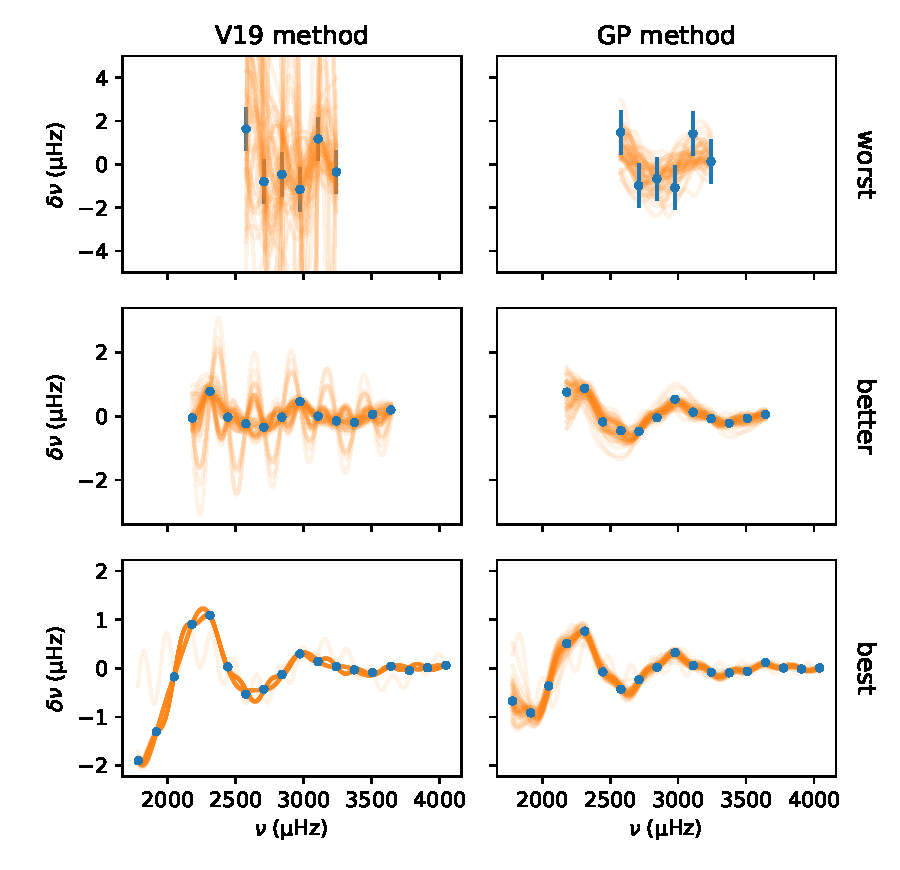
\includegraphics{figures/glitch-test-signal.pdf}
    \caption{50 random draws from the V19 and GP methods showing the total glitch signal, \(\delta\nu = \delta_\helium(\nu) + \delta_\bcz(\nu)\), as a function of frequency, \(\nu\). The data points plot in blue are the median smooth component model at \(\vect{n}\) subtracted from the observed modes \(\vect{\nu}_\obs\) with their observed uncertainty \(\sigma_\obs\).}
    \label{fig:glitch-test-signal}
\end{figure}

In Figure \ref{fig:glitch-test-signal}, we plot the predicted glitch component, \(\delta\nu\), using 50 draws from the posterior distribution on the model parameters for both methods. We subtracted the median background component from the observed \(\nu_n\) over-plot. For each scenario, both methods predicted similar median glitch components. However, the \citetalias{Verma.Raodeo.ea2019} method showed more extreme multimodality in all cases. For example, the better case showed a high-amplitude (\(\sim \SI{2}{\micro\hertz}\)) BCZ glitch solution which is not present with the GP method. Such a large signal would indicate a highly unlikely density discontinuity at the BCZ. Additionally, the two methods differed by \(\sim \SI{1}{\micro\hertz}\) at low frequency in the best case. Despite this, the \citetalias{Verma.Raodeo.ea2019} method appeared to be more confident in its glitch solutions compared to the GP method.

\begin{figure}[!tbp]
    \centering
    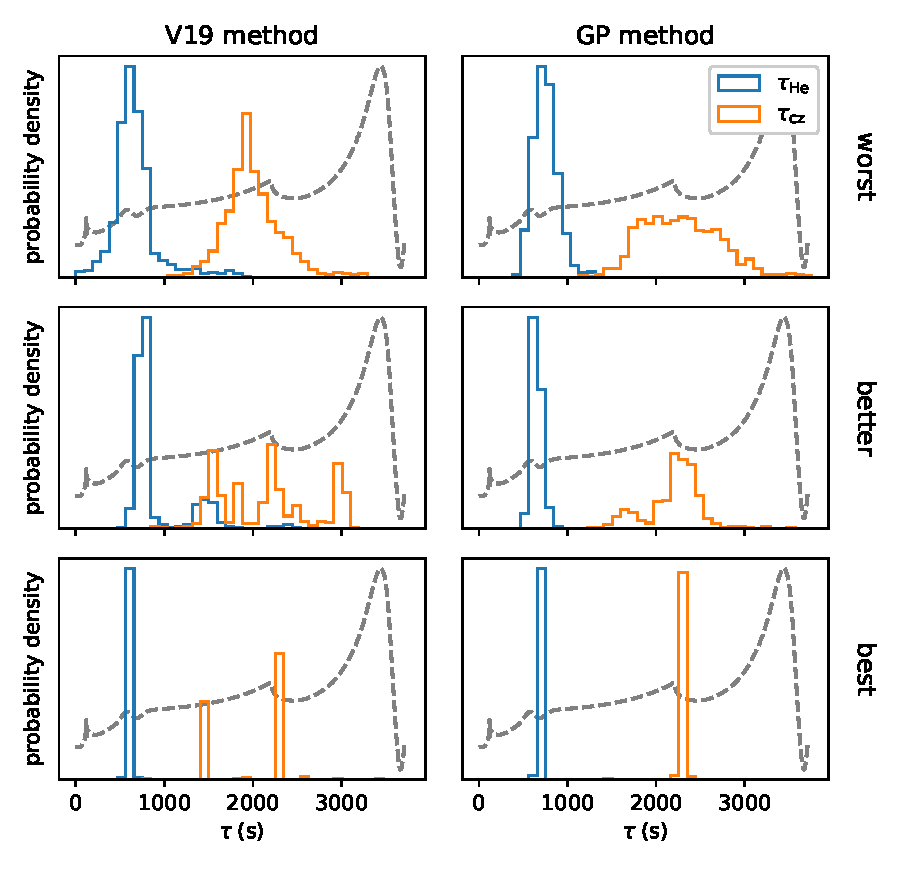
\includegraphics{figures/glitch-test-tau.pdf}
    \caption{Samples from the V19 and GP methods for the acoustic depths of the helium glitch (\(\tau_\helium\)) and base of the convective zone (\(\tau_\bcz\)). The sound-speed gradient from Figure \ref{fig:sound-speed-gradient} is over-plot with a grey dashed line.}
    \label{fig:glitch-test-tau}
\end{figure}

We plotted posterior distributions of the glitch acoustic depths, \(\tau_\helium\) and \(\tau_\bcz\), in Figure \ref{fig:glitch-test-tau} and compared them to the sound speed gradient of the test star from Figure \ref{fig:sound-speed-gradient}. We expect the acoustic depths to approximately line up with the sharp structural changes. For the worst case, both methods gave broad distributions for the acoustic depths, compatible with their respective initial guesses and priors. The \citetalias{Verma.Raodeo.ea2019} method initial guesses appeared to underestimate \(\tau_\bcz\), whereas the GP method prior was broad enough to encompass a wide range of possible \(\tau_\bcz\). In the better and best cases, we found that the \citetalias{Verma.Raodeo.ea2019} had strong multimodality. For example, the better case found solutions for \(\tau_\helium\) far deeper into the star than we would expect, at around \SI{1500}{\second} and \SI{2500}{\second}.

As predicted by \citet{Houdek.Gough2007} and shown in \citet{Verma.Faria.ea2014}, the the values for \(\tau_\helium\) obtained were under-predicted compared to the location of the trough due to the second ionisation of helium. This is because \(\delta\nu_\helium\) does not include the smaller glitch component due to the first ionisation of helium, located at a smaller \(\tau\). We can see this for the best star fit with the \citetalias{Verma.Raodeo.ea2019} method which finds \(\tau_\helium = \SI{619(15)}{\second}\). The depression in \(\gamma\) due to He\,\textsc{ii} ionisation in the respective stellar model is located at \SI{733}{\second}. On the other hand, the GP method was closer with \(\tau_\helium = \SI{696(19)}{\second}\).

\begin{figure}[!tb]
    \centering
    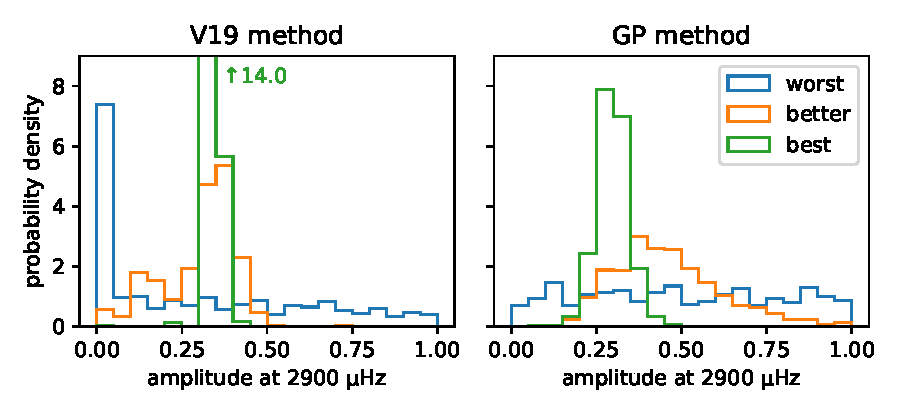
\includegraphics{figures/glitch-test-amplitude.pdf}
    \caption{Samples of the helium glitch amplitude at a reference frequency of \SI{3000}{\micro\hertz} fit with the V19 and GP methods for the worst-, better-, and best-case test data. The tallest bar in the V19 method panel is cropped with its value displayed in green text.}
    \label{fig:glitch-test-amplitude}
\end{figure}

We compared helium glitch amplitudes at \(\nu_\mathrm{ref}\) from both methods in Figure \ref{fig:glitch-test-amplitude}. The \citetalias{Verma.Raodeo.ea2019} method preferred low-amplitude solutions for the worst and better cases than the best case compared to the GP method. On the other hand, the GP method reflects our prior in the worst case, with the width of the distribution shrinking as the data improves. The GP method does show some bi-modality in the better case, with a solution at \(A_\helium^\mathrm{ref} \approx 0.7\) which was not found by the \citetalias{Verma.Raodeo.ea2019} method. In the best case, the \citetalias{Verma.Raodeo.ea2019} method obtained \(A_\helium^\mathrm{ref} = 0.347_{-0.005}^{+0.006}\), whereas the GP method found \(A_\helium^\mathrm{ref} = 0.296_{-0.036}^{+0.042}\).

% Why not use delta gamma / gamma as the probe of helium abundance? That is proportional to alpha / sqrt(beta). Then, an update to this method can use this and beta as a parameter and then work out alpha from that, since beta should scale with tau and the depth is a signature of helium abundance. Be careful as number of modes correlates with delta nu value of fit.

\subsubsection{16 Cyg A}

We compared the results from both methods applied to the 16 Cyg A data in Figure \ref{fig:glitch-16cyga}. We found that the \citetalias{Verma.Raodeo.ea2019} method predicted extreme solutions for the glitch where the GP method did not. There was also a difference of about \SI{1}{\micro\hertz} at the low frequency end such that the \citetalias{Verma.Raodeo.ea2019} predicted a larger glitch amplitude. Otherwise, the two methods gave similar predictions for the glitch function.

Both methods found similar values for \(\tau_\helium\) but relatively different distributions for \(\tau_\bcz\). Regarding the helium glitch, the \citetalias{Verma.Raodeo.ea2019} method found \(\tau_\helium = 917_{-53}^{+50} \, \mathrm{s}\), and our GP method obtained \(\tau_\helium = 931_{-88}^{+59} \, \mathrm{s}\), within 1-\(\sigma\) of each other. As seen in the previous section, our method found a slightly larger value of \(\tau_\helium\) than the \citetalias{Verma.Raodeo.ea2019} method, although not significantly in this case. \citet{Verma.Faria.ea2014} fit the glitch with \(l=0,1,2\) modes and found an acoustic depth of \SI{930(14)}{\second}, within 1-\(\sigma\) of both methods in this work.

We calculated the helium glitch amplitude at a reference frequency of \SI{2188.5}{\micro\hertz}, equivalent to the value of \(\nu_{\max}\) obtained by \citet{Lund.SilvaAguirre.ea2017}. Samples from both posteriors are shown in the bottom panel of Figure \ref{fig:glitch-16cyga}. We found \(A_\helium^\mathrm{ref} = 0.260_{-0.065}^{+0.050}\) for the \citetalias{Verma.Raodeo.ea2019} method, and \(A_\helium^\mathrm{ref} = 0.333_{-0.073}^{+0.081}\) for the GP method. Both values were about 1-\(\sigma\) apart. Additionally, both methods found \(A_\bcz^\mathrm{ref} \sim 0.1\), with the GP method favouring a smaller value. The \citetalias{Verma.Raodeo.ea2019} method found some solutions with \(A_\bcz^\mathrm{ref}\) larger than \(A_\helium^\mathrm{ref}\), something we would not expect because the modes are less sensitive to structural changes deeper in the star.

\begin{figure}[!tb]
    \centering
    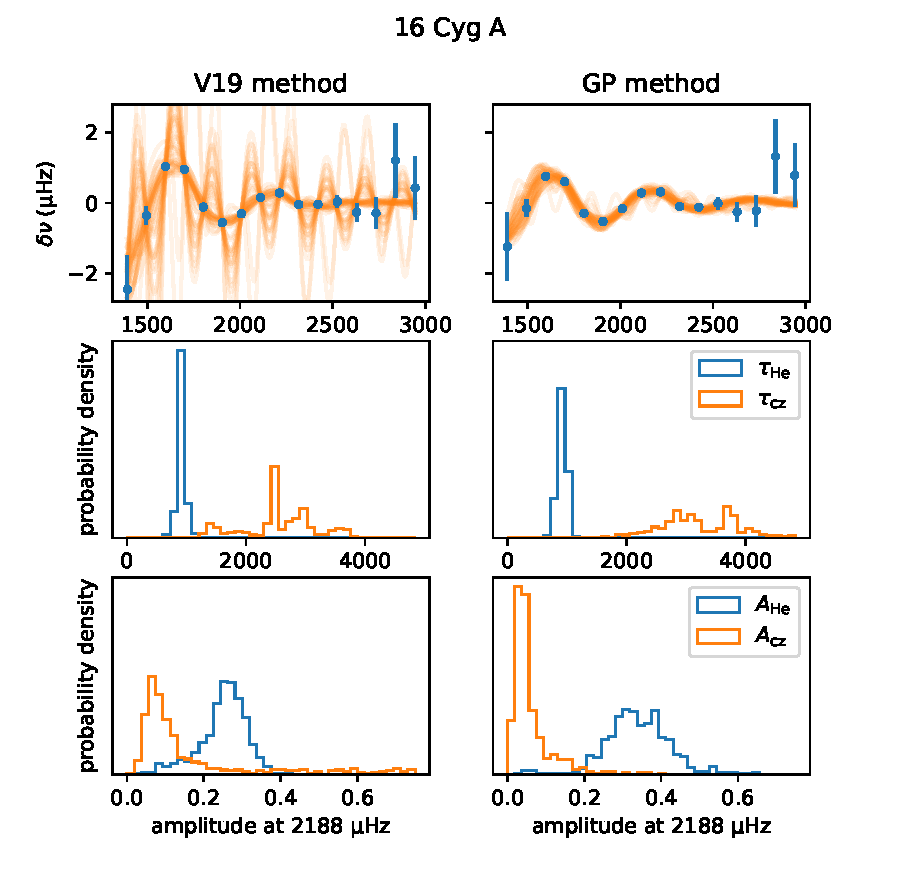
\includegraphics{figures/glitch-16cyga.pdf}
    \caption{Results for the glitch fit to 16 Cyg A using the \citetalias{Verma.Raodeo.ea2019} method (\emph{left}) and GP method (\emph{right}). The top panel shows 50 draws from the posterior prediction of \(\delta\nu = \delta\nu_\helium + \delta\nu_\bcz\) with the observed \(\nu_n\) minus the median smooth background component of the model. The middle and bottom panels shows the posterior sample probability density for the acoustic depths and reference amplitudes of the glitches respectively.}
    \label{fig:glitch-16cyga}
\end{figure}

\subsection{Discussion}\label{sec:glitch-disc}

% Discuss major differences

\begin{figure}[!tb]
    \centering
    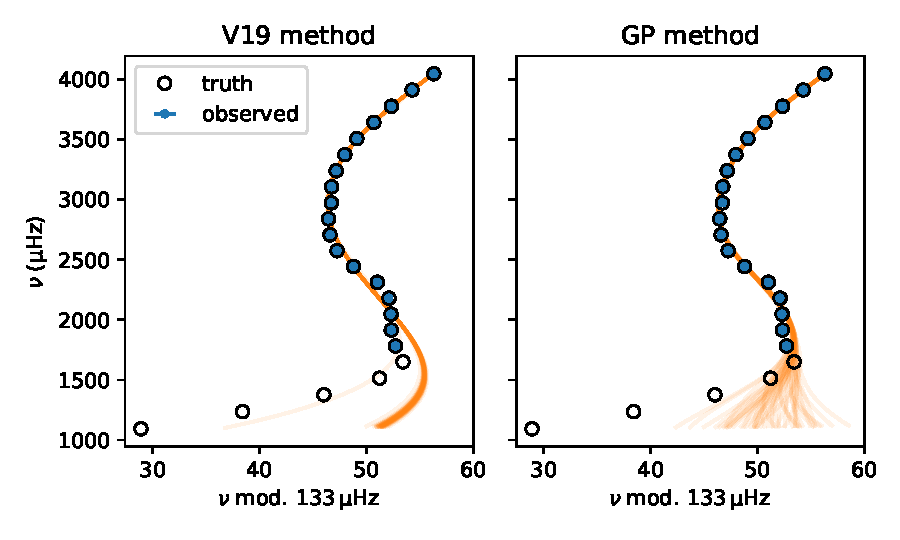
\includegraphics{figures/glitch-test-smooth.pdf}
    \caption{Echelle-like diagrams showing mode frequencies plot against their frequency modulo \SI{133}{\micro\hertz} for the best case scenario. The orange lines show 50 draws from the model posterior predictions with the glitch component removed (\(f(n) - \delta\nu\)) for both methods. The predictions are made from a lower radial order \(n=8\) than the observed modes. The true values from model S are shown for each mode. Some radial orders (\(n\)) are shown next to the modes for context.}
    \label{fig:best-smooth}
\end{figure}

Throughout this work, we found a smaller \(\delta\nu\) amplitude at low frequency with the GP method than with the \citetalias{Verma.Raodeo.ea2019} method. This was particularly visible in the best case and in 16 Cyg A. We expected this was a result of the different smooth background models. In Figure \ref{fig:best-smooth} we plotted the smooth component of each model extended to lower order, unobserved modes. We found the GP background component has a turning point at \(\nu \approx \SI{1900}{\micro\hertz}\), higher than the \citetalias{Verma.Raodeo.ea2019} method at \(\nu \approx \SI{1500}{\micro\hertz}\). The smooth component of the \citetalias{Verma.Raodeo.ea2019} method was confidently incorrect outside of the observed frequencies. Conversely, the GP method predicted closer to the truth with increasing uncertainty further from the observations. Therefore, it appears that the GP provided a more accurate representation of the true underlying function than the polynomial.

\begin{figure}[!tb]
    \centering
    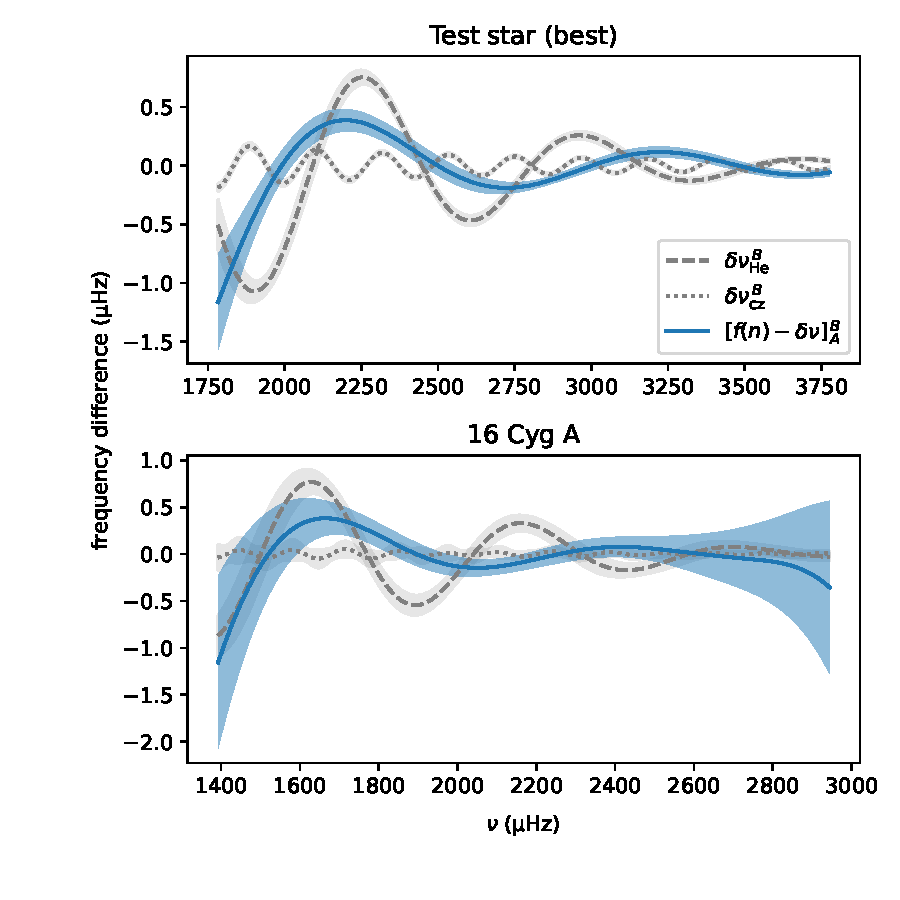
\includegraphics[trim={0.4in 0.2in 0 0},clip]{figures/glitch-res.pdf}
    \caption{The difference between the model without the glitch components (\(f(n) - \delta\nu\)) predicted by the \citetalias{Verma.Raodeo.ea2019} method (A) and the GP method (B). The glitch components from the GP method are plot in gray for context. The 68 per cent confidence region is shaded for each line.}
    \label{fig:smooth-res}
\end{figure}

In the test star's best case and 16 Cyg A, the GP method found a higher \(\tau_\helium\) than the \citetalias{Verma.Raodeo.ea2019} method. The GP was possibly better able to distinguish between He\,\textsc{i} and He\,\textsc{ii} ionisation compared to the polynomial. To verify this, we plotted the difference between each model's predictions with the glitch subtracted in Figure \ref{fig:smooth-res}. We saw a clear oscillatory signal in the differences. The period of this signal in the test star corresponded to an acoustic depth of \(\sim \SI{500}{\second}\), matching the location of He\,\textsc{i} ionisation in model S. The oscillatory signal was less pronounced for 16 Cyg A, but corresponded to a plausible He\,\textsc{i} acoustic depth of \(\sim \SI{700}{\second}\). The polynomial was not flexible enough to pick up this signal, thus lowering its inferred value for \(\tau_\helium\). As a result, the GP method more accurately determined the acoustic depth of the second helium ionisation zone.

% Discuss the prior

The \citetalias{Verma.Raodeo.ea2019} method found several extreme solutions for \(\delta\nu\) whereas GP method did not. We expected this because the GP method used a prior on the model parameters. We tested relaxing the prior on \(\vect{\theta}_B\) and recovered similar solutions to the \citetalias{Verma.Raodeo.ea2019} method, showing that the prior helped eliminate unrealistic solutions. Therefore, care should be taken over the choice of prior on \(\vect{\theta}_B\) to realistically reflect our expectation. If some of our prior assumptions are incorrect they may bias the results. For example, the outer convective region gets shallower as stars get hotter (approaching \(\teff \approx \SI{7000}{\kelvin}\)) making the assumption that \(\tau_\bcz/\tau_0 \approx 0.6\) an overestimate in these cases. We accommodate for this with a wide prior on \(\tau_\bcz\), but this could be improved. There is a notable temperature dependence to \(\tau_\bcz/\tau_0\) observed in the grid of stellar models which could be exploited in the future when constructing the prior.

Additionally, the samples for \(\alpha_\helium\) and \(\beta_\helium\) were correlated in both methods. This was expected, because larger values of \(\beta_\helium\) can be compensated for with a larger amplitude factor \(\alpha_\helium\). In the GP method, we did not include this expected correlation in our prior. Hence, we found that having broader priors on \(\alpha_\helium\) and \(\beta_\helium\) lead to the prior predicting unrealistic glitches. In future work, we could devise a multivariate prior for the amplitude parameters to account for this. However, we note that our approach still improves on the \citetalias{Verma.Raodeo.ea2019} method by using a prior.

A potential limitation of the GP method is that we calculate the glitch at \(\tilde{f}_B(n)\) from the linear asymptotic equation (Equation \ref{eq:asy}). In regions where the gradient of \(\delta(\nu)\) is high, the difference between \(\tilde{f}_B(n)\) and the true frequency can be up to (\(\sim \SI{0.1}{\micro\hertz}\)). The GP kernel function cannot absorb this difference because is varies on a short length-scale. Instead, we accounted for this uncertainty by adding Gaussian noise to the model parametrised by \(\sigma\). However, for the best test star, we found \(\sigma \approx 0.05\), which was larger than the observational uncertainty, \(\sigma_\obs = 0.01\). This could limit our method's inference ability for the best asteroseismic targets. One solution is to replace \(\tilde{f}_B(n)\) with a quadratic \citep[e.g.][]{Nielsen.Davies.ea2021} which better approximates \(\nu_n\). However, the GP kernel would need to be adjusted to account for this. We leave this for the next iteration of this method.

% Using the glitch parameters as a helium diagnostic could involve measuring the amplitude of the helium glitch at a reference frequency such as \(\nu_{\max}\). We should expect solutions for this reference amplitude (\(A_\mathrm{ref}\)) to converge on a value as the data quality increases from worst to best. It is also important that the uncertainty of the reference amplitude is accurate if using it to constrain helium abundance in a population of stars. If using V19 method on a population of stars, this could bias inference towards lower values of helium abundance.

\subsection{Conclusion}

We introduced a new method for modelling acoustic glitches in solar-like oscillators using a Gaussian Process. Testing the method on a model star, we found that it more accurately characterised the underlying, smoothly-varying functional form of the radial modes than the 
\citetalias{Verma.Raodeo.ea2019} method. Furthermore, our method was able to absorb the glitch component from He\,\textsc{i} ionisation, for which the polynomial was not flexible enough.

Additionally, the GP method provided more believable uncertainties on the glitch parameters, whereas the \citetalias{Verma.Raodeo.ea2019} method was over-confident with the best data and under-confident with the worst. This would become a problem if using the results to make further inference about helium enrichment. For example, the GP modelled correlated `noise' in the mode frequencies arising from He\,\textsc{i} ionisation, not possible with the polynomial in the \citetalias{Verma.Raodeo.ea2019} method. However, this raises the question of whether He\,\textsc{i} ionisation glitch should be included in the model --- this depends how much helium abundance is to be gained from its parameters.

Future development of the method could involve building a prior for the glitch parameters. For example, we could start with fitting the model to simulated stars and using the results to build an empirical prior. Then, we could run the model on the full LEGACY asteroseismic sample of main sequence stars \citep{Lund.SilvaAguirre.ea2017} and compare our results to those from \citet{Verma.Raodeo.ea2019}. Consequently, we can add parameters carrying information about helium abundance to the hierarchical model introduced in \citet{Lyttle.Davies.ea2021}. Ultimately, our goal is to scale this method to the \(\sim \num{1000}\) high signal-to-noise solar-like oscillators expected to be observed by \emph{PLATO} \citep{Rauer.Catala.ea2014}.

\todo{Conclusion feels a little rushed, revisit.}